% This is the manual for the GSS 0.46.
%
% Copyright (C) 2005, 2006 Gong Ding.
% Email : gdiso@ustc.edu
% Permission is granted to copy, distribute and/or modify this document
% under the terms of the GNU Free Documentation License, Version 1.1 or
% any later version published by the Free Software Foundation; with no
% Invariant Sections, with no Front-Cover Texts, and with no Back-Cover
% Texts.

\RequirePackage{ifpdf}
\ifpdf % We are running pdfTeX in pdf mode
\documentclass[11pt,pdftex]{article}
\else
\documentclass{article}
\fi

% Page layout.
\advance\textwidth by 1.1in
\advance\oddsidemargin by -.55in
\advance\evensidemargin by -.55in
%
\advance\textheight by 1in
\advance\topmargin by -.2in
\advance\footskip by -.2in
%
\pagestyle{headings}
%
% Avoid some overfull boxes.
\emergencystretch=.1\hsize \hbadness = 3000

% these are from lshort.sty, but lshort.sty pulls in so many other
% packages it seems cleaner to just include them here.
%
\newcommand{\bs}{\symbol{'134}}%Print backslash
\newcommand{\ci}[1]{\texttt{\bs#1}}

\makeatletter
\@ifpackageloaded{tex4ht}{%
  % separate definition for HTML case to avoid
  % nasty borders with double horizontal lines with
  % large gaps.
  \newsavebox{\cmdsyntaxbox}%
  \newenvironment{cmdsyntax}{%
    \par
    % \small
    \addvspace{3.2ex plus 0.8ex minus 0.2ex}%
    \vskip -\parskip
    \noindent
    \begin{lrbox}{\cmdsyntaxbox}%
      \begin{tabular}{l}%
        \rule{0pt}{1em}%
        \ignorespaces
  }{%
      \end{tabular}%
    \end{lrbox}%
    \fbox{\usebox{\cmdsyntaxbox}}%
    \par
    \nopagebreak
    \addvspace{3.2ex plus 0.8ex minus 0.2ex}%
    \vskip -\parskip
  }%
}{%
  \newenvironment{cmdsyntax}{%
    \par
    \small
    \addvspace{3.2ex plus 0.8ex minus 0.2ex}%
    \vskip -\parskip
    \noindent
    \begin{tabular}{|l|}%
      \hline
      \rule{0pt}{1em}%
      \ignorespaces
  }{%
      \\%
      \hline
    \end{tabular}%
    \par
    \nopagebreak
    \addvspace{3.2ex plus 0.8ex minus 0.2ex}%
    \vskip -\parskip
  }%
} \makeatother

\usepackage[pdftex]{graphicx}
\usepackage{flafter}
\usepackage{array,indentfirst,longtable,amsmath}
\usepackage[T1]{fontenc}


\def\Hanh{H\`an Th\^e\llap{\raise 0.5ex\hbox{\'{}}} Th\`anh}

\ifpdf
  \usepackage[%
    pdftex,%
    colorlinks,%
    hyperindex,%
    plainpages=false,%
    bookmarks=true,%
    bookmarksnumbered=true%
  ]{hyperref}
  %%?? \def\pdfBorderAttrs{/Border [0 0 0] } % No border arround Links
  \usepackage{thumbpdf}
\else
  \usepackage{hyperref}
\fi

\pdfinfo{
   /Title  (GSS User's Guide)
   /Subject(User's Guide of GSS-0.46)
   /Author (Gong Ding, gdiso@ustc.edu)
   /Keywords (GSS, TCAD, Semiconductor Simulation, DDM, HDM)
   /CreationDate (D:20061116120000)
   /ModDate (D:20070219120000)
}

\title{GSS User's Guide Ver 0.46.07}
\author{Gong Ding
    \\University of Science and Technology of China
    \\\centerline{
\includegraphics[scale=0.3]{USTCLogo.png}}
    \\Email: gdiso@ustc.edu
}


\begin{document}

% comes out too close to the toc, and we know it's page one anyway.
\thispagestyle{empty}
\maketitle
\tableofcontents
\setcounter{tocdepth}{2}% for bookmark levels

\section{Introduction}
\subsection{The format of input card}
Like PISCES and MEDICI, GSS takes its command cards from a user
specified disk file. The input is read by GSS's build-in command
parser. Each line is recognized as a particular statement,
identified by the first word (named as keyword) on the card. The
remaining parts of the line are the parameters of that keyword. The
statement has the format as follow:
\begin{verbatim}
            KEYWORD [parameters]
\end{verbatim}
The words on a line are separated by blanks or tabs. If more than
one line of input is necessary for a particular statement, it may be
continued on subsequent lines by placing a backslash sign
'\textbackslash' as the last non-blank character on the current
line. Parameters may be one of four types: float, integer, bool or
string. The float point number supports C style double precision
real number. The bool value can be True, On, False and Off. String
value is made up of lower line, dot, blank, number and alpha
characters. The string should not begin with number and quotation
marks are only needed if it contains blank. At last, the length of
string is limited to 31 characters. All the parameter specification
has the same format as
\begin{verbatim}
            parameter_name = [number|integer|bool|string]
\end{verbatim}


In the card descriptions, keywords and parameters are not case
sensitive. But user input strings do, because file name may be
specified by the string. Comments must begin with '\#' and can be
either an separated line or locate at the end of current statement.

\subsection{The sequence of input deck}
Most of the cards GSS used are sequence insensitive. The order of
occurrence of cards is significant in only two cases. The mesh
generation cards must have the right order, or it can't work
properly. GSS will execute the 'driven' cards sequently. So the
placement order of 'driven' cards will affect simulation result.

\subsection{Statement Description Format}
\subsubsection*{Syntax of Parameter Lists}
The following special characters are used in the formatted parameter
list:
\begin{verbatim}
        Angle brackets < >  - parameter type
        Square brackets [ ] - optional group
        Vertical bar |      - alternate choice
        Parentheses ( )     - group hierarchy
        Braces { }          - group hierarchy with high level
\end{verbatim}

\subsubsection*{Value Types}
Besides some string parameters which have fixed values, most of the
parameters need a user defined value. A lower case letter in angle
brackets represents a value of a given type. The following types of
values are represented:
\begin{verbatim}
        <n> - double precision numerical value
        <i> - integer value
        <b> - bool value
        <s> - string value
\end{verbatim}



\newpage
\section{Global Specification}
\subsection{SET}
\subsubsection*{Description} Some global definitions such as the unit scale
and environment temperature must be set before the initiation of
GSS's build-in data. The \textsf{SET} command will do the
definition.

\subsubsection*{Syntax}

\begin{verbatim}
        set Carrier=(p|n|pn)
        set Z.Width=<n>
        set LatticeTemp=<n>
        set DopingScale=<n>
\end{verbatim}

\small
\noindent\begin{longtable}{ccccp{7cm}}
\textbf{parameter}   & \textbf{type}          & \textbf{default} & \textbf{unit} & \textbf{description} \\
Carrier     & string  & pn   & -              & The \textbf{Carrier} parameter specifies whether single or dual
                                                carriers will be modeled during the simulation. But at present,
                                                GSS only supports dual carriers, so the parameter value must always be "pn" \\
Z.Width     & number  & 1    & $\mathrm{\mu m}$ & \textbf{Z.Width} is needed by current calculation. Because GSS
                                                is a two-dimensional simulator, the length in Z direction must be
                                                given if GSS simulates transistor with external circuit.  \\
LatticeTemp & number  & 300  & $\mathrm{K}$        & \textbf{LatticeTemp} defines external temperature.      \\
DopingScale & number  & 1e18 & $\mathrm{cm^{-3}}$  & \textbf{DopingScale} will effect GSS's inner unit scale procedure
                                                     which shows great influence to the convergence of nonlinear solver.
                                                     In most case, set this value to max(Nd,Na) is a good choice. But
                                                     sometimes, a smaller value may be better.\\
\end{longtable}
\normalsize

\subsubsection*{Example}
\begin{verbatim}
        set Carrier     = pn    # specify carrier type.
        set Z.Width     = 2     # device width in Z dimension. Unit:um
        set LatticeTemp = 3e2   # specify initial temperature of device. Unit:K
        set DopingScale = 1e16  # set carrier scale reference value
\end{verbatim}


\newpage
\section{Mesh Generation}
\subsection{Introduction}
The early version of GSS was designed as a pure solver. It uses
CGNS(CFD General Notation System) as semiconductor device model
file. This file format provides the ability to store grid, solution
data, material information, boundary condition and connectivity in a
single, well-defined and easy-to-use form. More important, CGNS has
been accepted and supported by most of the commercial CFD
corporations. So users have various ways to create their models. For
example, models can be created by SGFramework, converted from MEDICI
TIF file by TIFTOOL (shipped with GSS) or generated by ICEMCFD,
which is a commercial CFD pre-processor.

Until very recently, the PISCES like model description language had
been introduced to GSS. The mesh generation arithmetic works as
follows. First, GSS builds the rectangle skeleton mesh by the model
description statements; Then, GSS employs Triangle (developed by
Jonathan Richard Shewchuk) to form the triangulate mesh and output
the mesh to an initial CGNS file. At last, GSS reads the CGNS file
again, computes the doping profile and finishes the remaining
calculations.

Triangle uses delaunay arithmetic, which forms a high quality
isotropic mesh. At the same time, MEDICI uses quadtree arithmetic to
generate its mesh, which often gives a regular mesh but the mesh
quality may be poor near the irregular boundary.

\subsection{Coordinate System}
The mesh generator uses a Cartesian coordinate system, in which the
top horizontal line has the maximal y coordinate and left vertical
line has the minimal x coordinate.

Note: This setting is different from PISCES and its commercial
versions like MEDICI and ATLAS.

\newpage
\subsection{MESH}
This statement indicates the beginning of the mesh generator.
\subsubsection*{Syntax}
\begin{verbatim}
        MESH [ Type=<s> ] ModelFile=<s> [ Triangle=<s> ]
\end{verbatim}

\small
\noindent\begin{longtable}{ccccp{7cm}}
\textbf{parameter}   & \textbf{type}  & \textbf{default} & \textbf{unit} & \textbf{description} \\
Type        & string  & -    & -      & \textbf{Type} indicates which mesh generator is to be used.
                                        But at present it is useless since GSS only has one mesh generator. \\
ModelFile   & string  & -    & -      & \textbf{ModelFile} gives the name of temporary CGNS file. \\
Triangle    & string  & pzq30AD  & -  & \textbf{Triangle} passes parameters to Triangle code.
                                        The detailed description of this string can be found at Triangle's home page
                                        http://www.cs.cmu.edu/~quake/triangle.html.\\
\end{longtable}
\normalsize

\subsubsection*{Example}
\begin{verbatim}
            MESH Type=GSS ModelFile=pn.cgns Triangle="pzA"
\end{verbatim}


\newpage
\subsection{XMESH and YMESH}
The \textbf{XMESH} and \textbf{YMESH} cards specify the location of
lines of nodes in a rectangular mesh. The original mesh can be
modified by following mesh cards like \textbf{ELIMINATE} and
\textbf{SPREAD}.

\subsubsection*{Syntax}
\begin{verbatim}
        XMESH  { WIDTH=<n> | ( X.MIN=<n> X.MAX=<n> ) }
               { N.SPACES=<i> [RATIO=<n>] | H1=<n> [H2=<n>] }
        YMESH  { DEPTH=<n> | ( Y.MAX=<n> Y.MIN=<n> ) }
               { N.SPACES=<i> [RATIO=<n>] | H1=<n> [H2=<n>] }
\end{verbatim}

\small
\noindent\begin{longtable}{ccccp{7cm}}
\textbf{parameter}   & \textbf{type}  & \textbf{default} & \textbf{unit} & \textbf{description} \\
WIDTH       & number  & -    & $\mathrm{\mu m}$     & The distance of the grid section in x direction. \\
DEPTH       & number  & -    & $\mathrm{\mu m}$     & The distance of the grid section in y direction. \\
X.MIN       & number  & -    & $\mathrm{\mu m}$     & The x location of the left edge of the grid section.
                                                      synonym: \textbf{X.LEFT}. The value of \textbf{X.MIN} will be set to right
                                                      edge of the previous grid section automatically.\\
X.MAX       & number  & -    & $\mathrm{\mu m}$     & The x location of the right edge of the grid section.
                                                      synonym: \textbf{X.RIGHT}. \\
Y.MIN       & number  & -    & $\mathrm{\mu m}$     & The y location of the bottom edge of the grid section.
                                                      synonym: \textbf{Y.BOTTOM}. \\
Y.MAX       & number  & -    & $\mathrm{\mu m}$     & The y location of the top edge of the grid section.
                                                      synonym: \textbf{Y.TOP}. The value of \textbf{Y.MAX} will be set to bottom
                                                      edge of the previous grid section automatically.\\
N.SPACES    & integer & 1    & -                    & The number of grid spaces in the grid section.\\
RATIO       & number  & 1.0  & -                    & The ratio between the sizes of adjacent grid spaces in the grid
                                                      section. \textbf{RATIO} should usually lie between 0.667 and 1.5. \\
H1          & number  & -    & $\mathrm{\mu m}$     & The size of the grid space at the begin edge of the grid section.\\
H2          & number  & -    & $\mathrm{\mu m}$     & The size of the grid space at the end edge of the grid section.\\
\end{longtable}
\normalsize

\subsubsection*{Example}
\begin{verbatim}
            XMESH    X.MIN=0.0  X.MAX=0.50   N.SPACES=8
            YMESH    DEPTH=0.1  N.SPACES=8   RATIO=0.8
            YMESH    DEPTH=0.1  N.SPACES=20
            YMESH    DEPTH=0.6  H1=0.005  H2=0.050
\end{verbatim}


\newpage
\subsection{ELIMINATE}
The \textbf{ELIMINATE} statement eliminates mesh points along planes
in a rectangular grid over a specified volume. This statement is
useful for eliminating nodes in regions of the device structure
where the grid is more dense than necessary. Points along every
second line in the chosen direction within the chosen range are
removed, except the first and last line. Successive eliminations of
the same range remove points along every fourth line, eighth line,
and so on.

\subsubsection*{Syntax}
\begin{verbatim}
        ELIMINATE   { DIRECTION = (ROWS | COLUMNS) }
                    [ {X.MIN=<n> | IX.MIN=<i>} ] [ {X.MAX=<n> | IX.MAX=<i>} ]
                    [ {Y.MIN=<n> | IY.MAX=<i>} ] [ {Y.MAX=<n> | IY.MIN=<i>} ]
\end{verbatim}

\small
\noindent\begin{longtable}{ccccp{7cm}}
\textbf{parameter}   & \textbf{type}  & \textbf{default} & \textbf{unit} & \textbf{description} \\
DIRECTION   & string  & -       & -                    & Specifies that horizontal or vertical lines of nodes are eliminated. \\
X.MIN       & number  & XMIN    & $\mathrm{\mu m}$     & The minimum x location of the rectangular volume in which nodes are eliminated.
                                                         synonym: \textbf{X.LEFT}. \\
X.MAX       & number  & XMAX    & $\mathrm{\mu m}$     & The maximum x location of the rectangular volume in which nodes are eliminated.
                                                         synonym: \textbf{X.RIGHT}. \\
IX.MIN      & integer & 0       & -                    & The minimum x node index of the rectangular volume in which nodes are eliminated.
                                                         synonym: \textbf{IX.LEFT}.\\
IX.MAX      & integer & IXMAX-1 &-                     & The maximum x node index of the rectangular volume in which nodes are eliminated.
                                                         synonym: \textbf{IX.RIGHT}. \\
Y.MIN       & number  & YMIN    & $\mathrm{\mu m}$     & The minimum y location of the rectangular volume in which nodes are eliminated.
                                                         synonym: \textbf{Y.BOTTOM}. \\
Y.MAX       & number  & YMAX    & $\mathrm{\mu m}$     & The maximum y location of the rectangular volume in which nodes are eliminated.
                                                         synonym: \textbf{Y.TOP}. \\
IY.MIN      & integer & 0       & -                    & The minimum y node index of the rectangular volume in which nodes are eliminated.
                                                         synonym: \textbf{IY.TOP}. \\
IY.MAX      & integer & IYMAX-1 & -                    & The maximum y node index of the rectangular volume in which nodes are eliminated.
                                                         synonym: \textbf{IY.BOTTOM}.
\end{longtable}
\normalsize

\subsubsection*{Example}
\begin{verbatim}
            ELIMINATE    Direction=COLUMNS  Y.TOP=-1.0
            ELIMINATE    Direction=ROWS     IX.MAX=8
\end{verbatim}


\newpage
\subsection{SPREAD}
The \textbf{SPREAD} statement provides a way to adjust the y
position of nodes along grid lines parallel to the x-axis in a
rectangular mesh to follow surface and junction contours.

\subsubsection*{Syntax}
\begin{verbatim}
       SPREAD LOCATION=(LEFT|RIGHT) WIDTH=<n> UPPER=<i> LOWER=<i> [ENCROACH=<n>]
              { Y.LOWER=<n>  | (THICKNES=<n> [VOL.RAT=<n>]) }
              [GRADING=<n>]
\end{verbatim}

\small
\noindent\begin{longtable}{ccccp{7cm}}
\textbf{parameter}   & \textbf{type}  & \textbf{default} & \textbf{unit} & \textbf{description} \\
LOCATION    & string  & -       & -                    & Specifies which side of the grid is distorted. \\
WIDTH       & number  & 0.0     & $\mathrm{\mu m}$     & The width of the distorted region measured from the left or
                                                         right edge of the structure. \\
UPPER       & integer & 0       & -                    & The index of the upper y-grid line of the distorted region. \\
LOWER       & integer & 0       & -                    & The index of the lower y-grid line of the distorted region. \\
ENCROACH    & number  & 1.0     & -                    & The factor which defines the abruptness of the transition
                                                         between distorted and undistorted grid. The transition region
                                                         becomes more abrupt with smaller \textbf{ENCROACH} factors. The minimum
                                                         allowed value is 0.1. \\
Y.LOWER     & number & -        & $\mathrm{\mu m}$     & The vertical location in the distorted region where the line
                                                         specified by \textbf{LOWER} is moved. The grid line specified by
                                                         \textbf{UPPER} does not move if this parameter is specified. \\
THICKNESS   & number & -        & $\mathrm{\mu m}$     & The thickness of the distorted region. Specifying \textbf{THICKNESS}
                                                         usually causes the positions of both the \textbf{UPPER} and \textbf{LOWER}
                                                         grid lines to move. \\
VOL.RAT     & number & 0.44     & -                    & The ratio of the displacement of the lower grid line to the net
                                                         change in thickness. If \textbf{VOL.RAT} is 0, the location of the
                                                         lower grid line does not move. If \textbf{VOL.RAT} is 1, the upper
                                                         grid line does not move. \\
GRADING     & number  & 1.0      & -                   & The vertical grid spacing ratio in the distorted region between
                                                         the y-grid lines specified with \textbf{UPPER} and \textbf{LOWER}
                                                         The spacing grows or shrinks by
                                                         GRADING in each interval between lines. \textbf{GRADING} should
                                                         usually lie between 0.667 and 1.5.
\end{longtable}
\normalsize

\subsubsection*{Example}
\begin{verbatim}
            SPREAD    Location=Left  Width=0.625 Upper=0 Lower=2 Thickness=0.1
            SPREAD    Location=Right Width=0.625 Upper=0 Lower=2 Thickness=0.1
\end{verbatim}


\newpage
\subsection{REGION}
The \textbf{REGION} statement defines the location of materials in
the mesh. Currently, GSS supports following materials: null space
including Vacuum and Air; semiconductor material including Si, Ge,
GaAs, $\mathrm{Si}_{1-x}\mathrm{Ge}_x$,
$\mathrm{Al}_x\mathrm{Ga}_{1-x}\mathrm{As}$ and
$\mathrm{In}_x\mathrm{Ga}_{1-x}\mathrm{As}$; insulator material
including $\mathrm{SiO}_2$ and electrode region including Elec, Al
and PolySi.

\subsubsection*{Syntax}
\begin{verbatim}
   REGION Shape=Rectangle Label=<s> Material=<s>
          [ X.MOLE=<n> [ MOLE.SLOPE=<n> | MOLE.END=<n> ] MOLE.GRAD=(X.Linear|Y.Linear) ]
          [ {X.MIN=<n> | IX.MIN=<n>} ] [ {X.MAX=<n> | IX.MAX=<n>} ]
          [ {Y.MIN=<n> | IY.MIN=<n>} ] [ {Y.MAX=<n> | IY.MAX=<n>} ]
   REGION Shape=Ellipse Label=<s> Material=<s>
          {CentreX=<n> CentreY=<n> MajorRadii=<n> MinorRadii=<n> Theta=<n> Division=<i>}
\end{verbatim}

\small
\noindent\begin{longtable}{ccccp{8.5cm}}
\textbf{parameter}   & \textbf{type}  & \textbf{default} & \textbf{unit} & \textbf{description} \\
Shape       & string  & -       & -                    & Specifies the shape of the region. Can be Rectangle or Ellipse.\\
Label       & string  & -       & -                    & Specifies the identifier of this region, limited to 12 chars. \\
Material    & string  & -       & -                    & Specifies the material of the region. Material strings can be
                                                         Vacuum, Air, Si, Ge, GaAs, SiGe, AlGaAs, InGaAs, SiO2, Elec, Al and PolySi.\\
X.MOLE      & number  & 0.0     & -                    & The mole fraction to use in the region for compound materials.
                                                         For graded compounds, \textbf{X.MOLE} represents the initial
                                                         mole fraction at the left, top, or front edge of the region
                                                         depending on whether X.Linear, or Y.Linear, respectively,
                                                         is specified. \\
MOLE.SLOPE & number   & 0.0     & $\mathrm{\mu m}^{-1}$ & The slope of the mole fraction for graded compounds. If this
                                                         parameter is used, the mole fraction has a value of \textbf{X.MOLE}
                                                         at the left, top or front edge of the region and a value of
                                                         \textbf{X.MOLE} + width * \textbf{X.SLOPE} at the right, bottom or back
                                                         edge of the region, where width is the width or depth of the
                                                         region. \\
MOLE.END   & number   & 0.0     & -                     & The mole fraction for graded compounds at the right, bottom,
                                                          or backedge of the region depending on whether X.Linear,
                                                          or Y.Linear, respectively, is specified. \\
MOLE.GRAD  & string   & Y.Linear & -                    & Specifies that the mole fraction grading is in the x or y direction. \\
X.MIN       & number  & XMIN    & $\mathrm{\mu m}$     & The minimum x location of the region.
                                                         synonym: \textbf{X.LEFT}. \\
X.MAX       & number  & XMAX    & $\mathrm{\mu m}$     & The maximum x location of the region.
                                                         synonym: \textbf{X.RIGHT}. \\
IX.MIN      & integer & 0       & -                    & The minimum x node index of the region.
                                                         synonym: \textbf{IX.LEFT}.\\
IX.MAX      & integer & IXMAX-1 &-                     & The maximum x node index of the region.
                                                         synonym: \textbf{IX.RIGHT}. \\
Y.MIN       & number  & YMIN    & $\mathrm{\mu m}$     & The minimum y location of the region.
                                                         synonym: \textbf{Y.BOTTOM}. \\
Y.MAX       & number  & YMAX    & $\mathrm{\mu m}$     & The maximum y location of the region.
                                                         synonym: \textbf{Y.TOP}. \\
IY.MIN      & integer & 0       & -                    & The minimum y node index of the region.
                                                         synonym: \textbf{IY.TOP}. \\
IY.MAX      & integer & IYMAX-1 & -                    & The maximum y node index of the region.
                                                         synonym: \textbf{IY.BOTTOM}.\\
CentreX     & number  & 0.0     & $\mathrm{\mu m}$   & The x location of the center of ellipse. \\
CentreY     & number  & 0.0     & $\mathrm{\mu m}$   & The y location of the center of ellipse.\\
MajorRadii  & number  & 1.0     & $\mathrm{\mu m}$   & The length of the major radii of ellipse.\\
MinorRadii  & number  & MajorRadii     & $\mathrm{\mu m}$   & The length of the minor radii of ellipse.\\
Theta       & number  & 0.0     & degree               & The angle of the first division point located on the boundary of ellipse region.\\
Division    & integer & 12      & -                    & The number of points which divide the boundary of ellipse into small segments.
\end{longtable}
\normalsize

\subsubsection*{Example}
\begin{verbatim}
            REGION    Label=Si1   Material=Si    Y.TOP= 0.000  Y.BOTTOM=-0.100
            REGION    Label=SiGe1 Material=SiGe  Y.TOP=-0.100  Y.BOTTOM=-0.125 \
                      X.MOLE=0.0  Mole.End=0.2
            REGION    Label=Hole  Material=SiO2 Shape=Ellipse CentreX=2.0 CentreY=-0.5 \
                      Division=24 MajorRadii=0.3 MinorRadii=0.3
\end{verbatim}

\subsubsection*{Hint}
Several regions can be defined one by one. But users should be
careful that regions can't get cross each other. The situations
showed by Fig\ref{Region1} (A) and (B) are allowed, but (C) will
break the mesh generator of GSS. The ellipse region is used for
photon crystal simulation. By choosing different division number,
GSS can build triangle, rectangle, hexagon as well as ellipse
(circle). Fig\ref{Region2} shows different shapes of polygons build
by ellipse.
\begin{figure}[ht]
  \hfill
  \begin{minipage}[t]{.5\textwidth}
    \begin{center}
      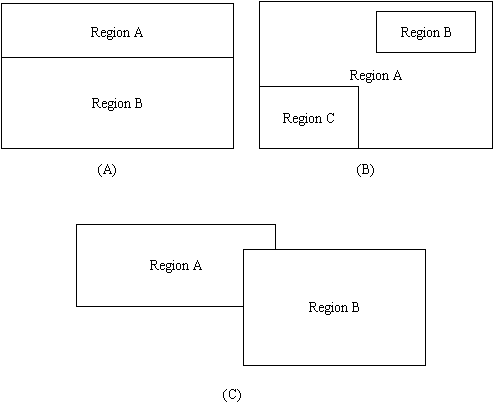
\includegraphics[scale=0.6]{r1.png}
      \caption{Multi-Region definition.}\label{Region1}
    \end{center}
  \end{minipage}
  \hfill
  \begin{minipage}[t]{.45\textwidth}
    \begin{center}
      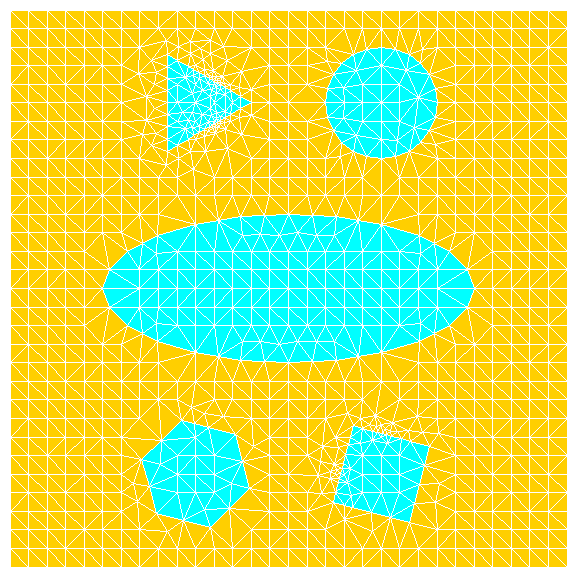
\includegraphics[scale=0.3]{region.png}
      \caption{Define shapes of ellipse region}\label{Region2}
    \end{center}
  \end{minipage}
  \hfill
\end{figure}

\newpage
\subsection{SEGMENT}
Segment is a group of boundary edges which have the same attribute.
This statement specifies the label of a special segment. User can
assign the segment with a special boundary type by \textbf{BOUNDARY}
statement.

\subsubsection*{Syntax}
\begin{verbatim}
       SEGMENT Label=<s> { Location=<s> | ( Direction=<s> X=<n> | Y=<n> ) }
               [ {X.MIN=<n> | IX.MIN=<n>} ] [ {X.MAX=<n> | IX.MAX=<n>} ]
               [ {Y.MIN=<n> | IY.MIN=<n>} ] [ {Y.MAX=<n> | IY.MAX=<n>} ]
\end{verbatim}

\small
\noindent\begin{longtable}{ccccp{7cm}}
\textbf{parameter}   & \textbf{type}  & \textbf{default} & \textbf{unit} & \textbf{description} \\
Label       & string  & -       & -                    & Specifies the identifier of this segment, limited to 31 chars. \\
Location    & string  & -       & -                    & Specifies which side the segment lies along. Allowed: TOP, BOTTOM, LEFT or RIGHT.\\
Direction   & string  & -       & -                    & Specifies the dimensional orientation of the segment. Allowed: Horizontal or Vertical. \\
X           & number  & 0.0     & $\mathrm{\mu m}$     & Specifies the X coordinate of the vertical segment. \\
Y           & number  & 0.0     & $\mathrm{\mu m}$     & Specifies the Y coordinate of the horizontal segment. \\
X.MIN       & number  & XMIN    & $\mathrm{\mu m}$     & The minimum x location of the segment.
                                                         synonym: \textbf{X.LEFT}. \\
X.MAX       & number  & XMAX    & $\mathrm{\mu m}$     & The maximum x location of the segment.
                                                         synonym: \textbf{X.RIGHT}. \\
IX.MIN      & integer & 0       & -                    & The minimum x node index of the segment.
                                                         synonym: \textbf{IX.LEFT}.\\
IX.MAX      & integer & IXMAX-1 &-                     & The maximum x node index of the segment.
                                                         synonym: \textbf{IX.RIGHT}. \\
Y.MIN       & number  & YMIN    & $\mathrm{\mu m}$     & The minimum y location of the segment.
                                                         synonym: \textbf{Y.BOTTOM}. \\
Y.MAX       & number  & YMAX    & $\mathrm{\mu m}$     & The maximum y location of the segment.
                                                         synonym: \textbf{Y.TOP}. \\
IY.MIN      & integer & 0       & -                    & The minimum y node index of the segment.
                                                         synonym: \textbf{IY.TOP}. \\
IY.MAX      & integer & IYMAX-1 & -                    & The maximum y node index of the segment.
                                                         synonym: \textbf{IY.BOTTOM}.
\end{longtable}
\normalsize

\subsubsection*{Example}
\begin{verbatim}
            SEGMENT   Label=Anode    Direction=Horizontal X.MIN=0.0 X.MAX=1.0 Y=0.0
            SEGMENT   Label=Cathode  Direction=Horizontal X.MIN=0.0 X.MAX=3.0 Y=-3.0
            SEGMENT   Label=Anode    Location=TOP   X.MIN=0.0 X.MAX=1.0
            SEGMENT   Label=Cathode  Location=BOTTOM
\end{verbatim}

\subsubsection*{Hint}
Here, I have to mention the naming principle of segments. Beside
labeled segments, the interface edges between two regions will be
assigned by IF\_\textit{name1}\_to\_\textit{name2} in which the
\textit{name1} and \textit{name2} is the labels of the two regions
by alpha order. The remain edges of a region will be assigned by
\textit{name}\_Neumann and the \textit{name} is the label of the
region.

One can define a segment for probing data. Please refer to \textbf{PROBE} statement.
This kind of segment should be placed inside a region. Equally, NO intersection to any other segment.

\newpage
\subsection{REFINE}
The \textbf{REFINE} statement allows refinement of a coarse mesh.

\subsubsection*{Syntax}
\begin{verbatim}
       REFINE  Variable=(Doping|Potential) Dispersion=<n> DivisionRatio=<n>
               [ Measure=(Linear|SignedLog) ] [ Triangle=<s> ]
\end{verbatim}

\small \noindent\begin{longtable}{ccccp{7cm}}
\textbf{parameter}   & \textbf{type}  & \textbf{default} & \textbf{unit} & \textbf{description} \\
Variable    & string  & -       & -   & Specifies that the grid refinement is based on the potential or doping quantity. \\
Measure     & string  & Linear  & -   & Specifies that refinement is based on the original value or logarithm of the
                                        specified quantity.\\
Dispersion  & number  & 3.0     & -   & The numerical criterion for refining a triangle. If the specified
                                        quantity differs by more than this parameter at the nodes of a triangle,
                                        the triangle is divided.\\
DivisionRatio & number & 0.25   & -   & The area of divided triangle over area of original triangle.
                                        The default value suggests Triangle code divide one triangle into 4 small triangles.
                                        It is a suggestion value, Triangle code will adjust it for mesh quality reason.\\
Triangle    & string  &praq30Dz & -   & Passes parameters to Triangle code.\\
\end{longtable}
\normalsize

\subsubsection*{Example}
\begin{verbatim}
            REFINE   Variable=Doping Measure=SignedLog Dispersion=1
            REFINE   Variable=Potential Measure=Linear Dispersion=0.1
\end{verbatim}

\begin{figure}[ht]
\centering
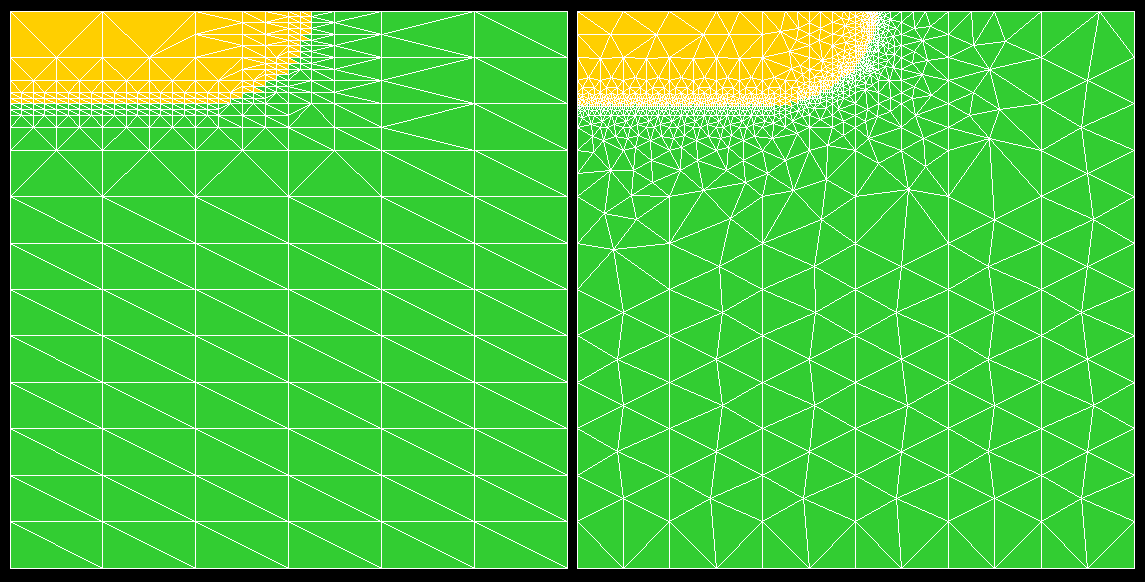
\includegraphics[scale=0.3]{refine.png}
\caption{Mesh refinement for a PN diode.}
\end{figure}

\newpage
\section{Doping Profile}
The \textbf{PROFILE} statement defines profiles for impurities to be
used in the device structure. At present, GSS supports analytic
profiles such as uniform, gauss distribution in both x-y directions
and error function distribution in x direction while gauss
distribution in y direction.

\subsubsection*{Syntax}
\begin{verbatim}
       PROFILE { Type=Uniform   |
                 Type=Gauss     [YCHAR=<n> | Y.Junction=<n>] [XCHAR=<n>] |
                 Type=ErrorFunc [YCHAR=<n>] [XCHAR=<n>] }
               Ion=(Donor|Acceptor) { N.Peak=<n> | Dose=<n> }
               [ X.MIN=<n> ] [ X.MAX=<n> ] [ Y.MIN=<n> ] [ Y.MAX=<n> ]
\end{verbatim}

\small
\noindent\begin{longtable}{ccccp{7cm}}
\textbf{parameter}   & \textbf{type}  & \textbf{default} & \textbf{unit} & \textbf{description} \\
Type        & string  & -       & -                    & Specifies that the profile has a uniform, gauss or error function distribution.\\
Ion         & string  & -       & -                    & Specifies the impurity ionization. \\
N.Peak      & number  & 0.0     & $cm^{-3}$            & The peak impurity concentration for an impurity profile.\\
Dose        & number  & 0.0     & $cm^{-2}$            & The dose of the impurity profile assuming a full Gaussian distribution.\\
X.MIN       & number  & 0.0     & $\mathrm{\mu m}$     & The minimum x location of the doping profile.
                                                         synonym: \textbf{X.LEFT}. \\
X.MAX       & number  & XMIN    & $\mathrm{\mu m}$     & The maximum x location of the doping profile.
                                                         synonym: \textbf{X.RIGHT}. \\
Y.MIN       & number  & YMAX    & $\mathrm{\mu m}$     & The minimum y location of the doping profile.
                                                         synonym: \textbf{Y.BOTTOM}. \\
Y.MAX       & number  & 0.0     & $\mathrm{\mu m}$     & The maximum y location of the doping profile.
                                                         synonym: \textbf{Y.TOP}. \\
YCHAR       & number  & 0.25    & $\mathrm{\mu m}$     & The y characteristic length of the profile outside the range of
                                                         \textbf{Y.MIN} < y < \textbf{Y.MAX}. \\
XCHAR       & number  & 0.25    & $\mathrm{\mu m}$     & The x characteristic length of the profile outside the range of
                                                         \textbf{X.MIN} < x < \textbf{X.MAX}. \\
Y.Junction  & number  & 0.0     & $\mathrm{\mu m}$     & The y location under the center of the profile where the magnitude
                                                         of the profile being added equals the magnitude of the
                                                         background profile. \\
\end{longtable}
\normalsize

\subsubsection*{Example}
\begin{verbatim}
        PROFILE   Type=Uniform Ion=Donor     N.PEAK=1E15 \
                  X.MIN=0.0 X.MAX=3.0  Y.TOP=0.0 Y.BOTTOM=-3.0
        PROFILE   Type=Gauss   Ion=Acceptor  N.PEAK=1E18 X.CHAR=0.2 Y.JUNCTION=-0.5 \
                  X.MIN=0.0 X.MAX=0.7  Y.TOP=0.0 Y.BOTTOM=0.0
        PROFILE   Type=ErrorFunc Ion=Acceptor  N.PEAK=2E17 X.CHAR=0.25 Y.CHAR=0.25 \
                  X.MIN=0.5 X.MAX=1.0  Y.TOP=0.0 Y.BOTTOM=0.0
\end{verbatim}


\newpage
\section{Voltage and Current Source}
\subsection{Introduction}
For simulation the transient response of device, GSS supports
several types of voltage and current source. The original models of
these sources come from SPICE, a famous circuit simulation program.
Several sources may be defined in one disk file. And the placement
of these definitions are not critical. The sources can be assigned
to electrode by \textbf{ATTACH} statement when needed.

\subsection{ISOURCE}

\subsubsection*{Syntax}
\begin{verbatim}
        isource Type=IDC  ID=<s> Tdelay=<n> Iconst=<n>
        isource Type=ISIN ID=<s> Tdelay=<n> Iamp=<n> Freq=<n>
        isource Type=IEXP ID=<s> Tdelay=<n> TRC=<n>  TFD=<n>
                TFC=<n> Ilo=<n> Ihi=<n>
        isource Type=IPULSE ID=<s> Tdelay=<n> Tr=<n> Tf=<n>
                Pw=<n> Pr=<n> Ilo=<n> Ihi=<n>
        isource Type=ISHELL ID=<s> DLL=<s> Func=<s>
\end{verbatim}

\small
\noindent\begin{longtable}{ccccp{7cm}}
\textbf{parameter}   & \textbf{type}    & \textbf{default} & \textbf{unit} & \textbf{description} \\
Type   & string  & -  & -    & This parameter declares which type of current source is defined here.
                               Only four types of current source listed as previous are supported at present. \\
ID     & string  & -  & -    & A unique string which identifies the current source.\\
Tdelay & number  & 0  & $\mathrm{s}$  & A proper delay time before the activation of this current source. \\
Iconst & number  & 0  & $\mathrm{mA}$ & The current of the IDC. \\
Iamp   & number  & 0  & $\mathrm{mA}$ & The amplitude current of the ISIN. \\
Freq   & number  & 0  & $\mathrm{Hz}$ & The frequency of the ISIN. \\
TRC    & number  & 0  & $\mathrm{s}$  & The rise time constant of the IEXP. \\
TFD    & number  & 0  & $\mathrm{s}$  & The fall delay time of the IEXP. \\
TFC    & number  & 0  & $\mathrm{s}$  & The fall time constant of the IEXP. \\
Tr     & number  & 0  & $\mathrm{s}$  & The raise edge of the IPULSE. \\
Tf     & number  & 0  & $\mathrm{s}$  & The fall edge of the IPULSE. \\
Pw     & number  & 0  & $\mathrm{s}$  & The pulse with of the IPULSE. \\
Pr     & number  & 0  & $\mathrm{s}$  & The period of the IPULSE. \\
Ilo    & number  & 0  & $\mathrm{mA}$ & The low current for both IEXP and IPULSE. \\
Ihi    & number  & 0  & $\mathrm{mA}$ & The high current for both IEXP and IPULSE. \\
DLL    & string  & -  & -             & The name of dynamic library file.\\
Func   & string  & -  & -             & The name of the function loaded from dynamic library file.
\end{longtable}
\normalsize

\subsubsection*{Example}
\begin{verbatim}
        isource Type=IDC    ID=I1 Tdelay=0 Iconst=5
        isource Type=ISIN   ID=I2 Tdelay=0 Iamp=0.1 Freq=1e6
        isource Type=IEXP   ID=I3 Tdelay=0 TRC=1E-6 TFD=3E-6 TFC=1E-6 Ilo=0 Ihi=1
        isource Type=IPULSE ID=I4 Tdelay=0 Tr=1E-9 Tf=1E-9 Pw=5E-6 Pr=1E-5 Ilo=0 Ihi=1
\end{verbatim}

\newpage
\subsection{VSOURCE}
\subsubsection*{Syntax}

\begin{verbatim}
        vsource Type=VDC  ID=<s> Tdelay=<n> Vconst=<n>
        vsource Type=VSIN ID=<s> Tdelay=<n> Vconst=<n> Vamp=<n> Freq=<n> Alpha=<n>
        vsource Type=VEXP ID=<s> Tdelay=<n> TRC=<n>  TFD=<n>
                TFC=<n> Vlo=<n> Vhi=<n>
        vsource Type=VPULSE ID=<s> Tdelay=<n> Tr=<n> Tf=<n>
                Pw=<n> Pr=<n> Vlo=<n> Vhi=<n>
        vsource Type=VSHELL ID=<s> DLL=<s> Func=<s>
\end{verbatim}

\small
\noindent\begin{longtable}{ccccp{7cm}}
\textbf{parameter}   & \textbf{type}  & \textbf{default} & \textbf{unit} & \textbf{description} \\
Type   & string  & -  & -             & This parameter declares which type of
                                        voltage source is defined here.
                                        Only four types of voltage source listed as previous are supported at present. \\
ID     & string  & -  & -             & A unique string which identifies the voltage source.\\
Tdelay & number  & 0  & $\mathrm{s}$  & A proper delay time before the activation of this voltage source. \\
Vconst & number  & 0  & $\mathrm{V}$  & The voltage of the VDC. \\
Vamp   & number  & 0  & $\mathrm{V}$  & The amplitude voltage of the VSIN. \\
Freq   & number  & 0  & $\mathrm{Hz}$ & The frequency of the VSIN. \\
Alpha  & number  & 0  & -             & The exponential attenuation parameter of the VSIN. \\
TRC    & number  & 0  & $\mathrm{s}$  & The rise time constant of the VEXP. \\
TFD    & number  & 0  & $\mathrm{s}$  & The fall delay time of the VEXP. \\
TFC    & number  & 0  & $\mathrm{s}$  & The fall time constant of the VEXP. \\
Tr     & number  & 0  & $\mathrm{s}$  & The raise edge of the VPULSE. \\
Tf     & number  & 0  & $\mathrm{s}$  & The fall edge of the VPULSE. \\
Pw     & number  & 0  & $\mathrm{s}$  & The pulse with of the VPULSE. \\
Pr     & number  & 0  & $\mathrm{s}$  & The period of the VPULSE. \\
Vlo    & number  & 0  & $\mathrm{V}$  & The low voltage for both VEXP and VPULSE. \\
Vhi    & number  & 0  & $\mathrm{V}$  & The high voltage for both VEXP and VPULSE. \\
DLL    & string  & -  & -             & The name of dynamic library file.\\
Func   & string  & -  & -             & The name of the function loaded from dynamic library file.
\end{longtable}
\normalsize

\subsubsection*{Example}
\begin{verbatim}
        vsource Type=VDC    ID=GND  Tdelay=0 Vconst=0
        vsource Type=VDC    ID=VCC  Tdelay=0 Vconst=5
        vsource Type=VSIN   ID=Vs   Tdelay=1e-6 Vamp=0.1 Freq=1e6
        vsource Type=VEXP   ID=V1   Tdelay=0 TRC=1e-6 TFD=1e-6 TFC=1e-6 Vlo=0 Vhi=1
        vsource Type=VPULSE ID=V2   Tdelay=0 Tr=1e-9 Tf=1e-9 Pw=5e-6 Pr=1e-5 Vlo=0 Vhi=1
        vsource Type=VSHELL ID=VGauss  DLL=foo.so Func=vsrc_gauss
\end{verbatim}

\newpage
\subsubsection*{Hint}
GSS supports user defined voltage and current source by loading
shared object (.so) file. The file which contains a user defined
voltage source should have the function as follow. GSS will pass the
argument time in the unit of second to the function
\textit{vsrc\_name} and get voltage value in the unit of volt. The
current source function is almost the same except the unit of
current is $\mathrm{mA}$.

\begin{verbatim}
    double vsrc_name(double time)
    {
       /* calculate the voltage amplitude */
       return vsrc_amplitude;
    }
    double isrc_name(double time)
    {
       /* calculate the current amplitude */
       return isrc_amplitude;
    }
\end{verbatim}

The c code should be linked with -shared and -fPIC option as:
\begin{verbatim}
    gcc -shared -fPIC -o foo.so foo.c -lm
\end{verbatim}

The \textit{foo.so} file should be put in the same directory as
input file.

\newpage
\section{Boundary Condition}

\subsection{BOUNDARY and CONTACT}
The \textbf{BOUNDARY} statement sets boundary information to
representing segments which defined by mesh generator or read from
CGNS file.

GSS now fully support electrode region (the material of this region
may be metal or poly-Si). One should use \textbf{CONTACT} statement
to specify the electrode type of this region(s).

\subsubsection*{Syntax}
\begin{verbatim}
        BOUNDARY Type=OhmicContact       ID=<s>  [ Res=<n> ] [ Cap=<n> ] [ Ind=<n> ]
                 [ Heat.Transfer=<n> ] [EXT.Temp=<n> ] [ConnectTo=<s>]
        BOUNDARY Type=SchottkyContact    ID=<s>  [ Res=<n> ] [ Cap=<n> ] [ Ind=<n> ]
                 WorkFunction=<n> [ Heat.Transfer=<n> ] [EXT.Temp=<n> ]
        BOUNDARY Type=GateContact        ID=<s>  WorkFunction=<n>
                 [ Res=<n> ] [ Cap=<n> ] [ Ind=<n> ]
                 [ Heat.Transfer=<n> ] [EXT.Temp=<n> ]
        BOUNDARY Type=InsulatorContact   ID=<s>  WorkFunction=<n> [ QF=<n> ]
                 [ Res=<n> ] [ Cap=<n> ] [ Ind=<n> ]
                 Thickness=<n> Eps=<n>  [ Heat.Transfer=<n> ] [EXT.Temp=<n> ]
        BOUNDARY Type=InsulatorInterface ID=<s>  [ QF=<n> ]
        BOUNDARY Type=Heterojunction     ID=<s>  [ QF=<n> ]
        BOUNDARY Type=NeumannBoundary    ID=<s> [ Heat.Transfer=<n> ] [EXT.Temp=<n> ]

        CONTACT  Type=OhmicContact       ID=<s>
                 [ Res=<n> ] [ Cap=<n> ] [ Ind=<n> ] [ConnectTo=<s>]
                 [ Heat.Transfer=<n> ] [EXT.Temp=<n> ]
        CONTACT  Type=SchottkyContact    ID=<s>
                 [ Res=<n> ] [ Cap=<n> ] [ Ind=<n> ]
                 WorkFunction=<n> [ Heat.Transfer=<n> ] [EXT.Temp=<n> ]
        CONTACT  Type=GateContact        ID=<s>  WorkFunction=<n>
                 [ Res=<n> ] [ Cap=<n> ] [ Ind=<n> ]
                 [ Heat.Transfer=<n> ] [EXT.Temp=<n> ]
        CONTACT  Type=FloatMetal         ID=<s>  [ QF=<n> ]
\end{verbatim}

\small
\noindent\begin{longtable}{ccccp{7cm}}
\textbf{parameter}   & \textbf{type}    & \textbf{default} & \textbf{unit} & \textbf{description} \\
Type          & string  & -  & -    & This parameter declares which type of boundary condition is defined here.\\
ID            & string  & -  & -    & A unique string which identifies the corresponding segment.\\
Res           & number  & 0  & $\Omega$      & The lumped resistance for the electrode.  \\
Cap           & number  & 0  & $\mathrm{F}$  & The lumped capacitance for the electrode. \\
Ind           & number  & 0  & $\mathrm{H}$  & The lumped inductance for the electrode. \\
ConnectTo     & string  & -  & -             & Specifies the ID of an ohmic electrode which connect to this ohmic electrode. Useful for CMOS structure.\\
WorkFunction  & number  &4.7 & $\mathrm{V}$  & The workfunction of the Schottky contact or gate material. \\
QF            & number  & 0  & $\mathrm{C}\cdot \mathrm{cm}^{-2}$  & For InsulatorContact and InsulatorInterface bc: The surface charge density of semiconductor-insulator interface. \\
QF            & number  & 0  & $\mathrm{C}\cdot \mathrm{cm}^{-2}$  & For Heterojunction bc: The surface charge density of heterojunction. \\
QF            & number  & 0  & $\mathrm{C}\cdot \mathrm{\mu m}^{-1}$  & For FloatMetal bc: The free charge per micron in Z dimension. \\
Thickness     & number  &2e-7  & $\mathrm{cm}$ & The thickness of $\mathrm{SiO}_2$ layer. \\
Eps           & number  &3.9   & -             & The relative permittivity of $\mathrm{SiO}_2$ layer.\\
Heat.Transfer & number  &1e3   &$\mathrm{W}/(\mathrm{cm}\cdot \mathrm{K})$   & The heat transfer rate of boundary. \\
EXT.Temp      & number  & LatticeTemp  & $\mathrm{K}$   & The external temperature. \\
\end{longtable}
\normalsize

\subsubsection*{Example}
\begin{verbatim}
        BOUNDARY Type=InsulatorContract  ID=SiSiO2    Res=0 Cap=0 Ind=0 \
                 Thickness=1e-6 Eps=3.9 WorkFunction=4.7 QF=0
        BOUNDARY Type=InsulatorInterface ID=IFACE     QF=0
        BOUNDARY Type=GateContract       ID=GATE      Res=0 Cap=0 Ind=0 WorkFunction=4.7
        BOUNDARY Type=NeumannBoundary    ID=WALL      Heat.Transfer=0 EXT.Temp=300
        BOUNDARY Type=SchottkyContract   ID=sgate     Res=0 Cap=0 Ind=0 VBarrier=0.8
        BOUNDARY Type=OhmicContract      ID=OMANODE   Res=0 Cap=0 Ind=0
        BOUNDARY Type=OhmicContract      ID=OMCATHODE Res=0 Cap=0 Ind=0
\end{verbatim}

\subsubsection*{Hint}
Four "electrode" boundary conditions are supported by GSS. The names
are ended with "Contact". The OhmicContact and SchottkyContact
electrodes have current flow in both steady state and transient
situations. While GateContact and InsulatorContact(a simplified
MOSFET Gate boundary condition) only have displacement current in
transient situation.

GSS supports five interfaces which can be set automatically:
semiconductor-insulator interface(InsulatorInterface),
semiconductor-electrode interface(set to OhmicContract as default),
interface between different semiconductor material(Heterojunction)
and  interface between same semiconductor material(Homojunction).
These boundaries can be set automatically by GSS if user didn't set
them explicitly. However, the electrode-insulator interface, may
have several situations: Gate to Oxide interface, FloatMetal to
Oxide interface or Source/Drain electrode to Oxide interface. As a
result, this interface can only be set correctly when electrode type
is known. Please refer to the following \textbf{CONTACT} statement.

GSS can build region with metal or poly-Si material to form an
electrode. Which means, i.e. for OhmicContact bc, one can simply
specify a segment as Ohmic bc or build an electrode region as Ohmic
electrode. Since Version 0.45.03, GSS considers electrode region,
semiconductor region and insulator region during calculation. As a
result, GSS added \textbf{CONTACT} statement for fast boundaries
specification of electrode region. At present, GSS support electrode
with the type of Ohmic, Schottky, Gate and FloatMetal. All the
electrode should be specified explicitly and GSS will set
corresponding boundaries automatically.

The "ID" parameter of \textbf{BOUNDARY} statement is limited to
segment label. And The "ID" parameter of \textbf{CONTACT} statement
is limited to region name.

The NeumannBoundary, which is the default boundary type for all the
non-interface segments, can also be set automatically.

\newpage
\subsection{ATTACH}
This statement is used to add voltage or current sources to the
electrode boundary. The statement first clears all the sources
connected to the specified electrode and then adds source(s) defined
by VApp or IApp parameter. If two or more sources are attached to
the same electrode, the total effect is the summation of all
sources. However, the sources attached to one electrode must have
the same type.

\subsubsection*{Syntax}
\begin{verbatim}
        ATTACH Electrode=<s>  Type=Voltage VApp=<s> [VApp=<s> ...]
        ATTACH Electrode=<s>  Type=Current IApp=<s> [IApp=<s> ...]
\end{verbatim}

\small \noindent\begin{longtable}{ccccp{7cm}}
\textbf{parameter}   & \textbf{type}    & \textbf{default} & \textbf{unit} & \textbf{description} \\
Electrode     & string  & -  & -    & Specifies which electrode boundary is to be attached with one or more sources.\\
Type          & string  & Voltage  & -    & The sources are voltage or current type.\\
VApp          & string  & -  & -    & Specifies the ID of voltage source which is to be attached to this electrode.\\
IApp          & string  & -  & -    & Specifies the ID of current source which is to be attached to this electrode.\\
\end{longtable}
\normalsize

\subsubsection*{Example}
\begin{verbatim}
        ATTACH   Electrode=Collector VApp=VCC
        ATTACH   Electrode=Emitter   VApp=GND
        ATTACH   Electrode=Base      VApp=Vb  VApp=Vs
        ATTACH   Electrode=Base      Type=Current  IApp=Ib  IApp=Is
\end{verbatim}

\subsubsection*{Hint}
If electrode is attached with voltage source(s), the R, C and L
defined by \textbf{BOUNDARY} statement will affect later simulation.
But solver will ignore those lumped elements with the electrode
which stimulated by current source(s). Please refer to Fig
\ref{Electrode}.

The positive direction of current is flow into the electrode.

Only Ohmic and Schottky electrodes can be attached by current
source(s).

If no source attached explicitly, the electrode is set to be
attached to ground.

\begin{figure}[ht]
\centering
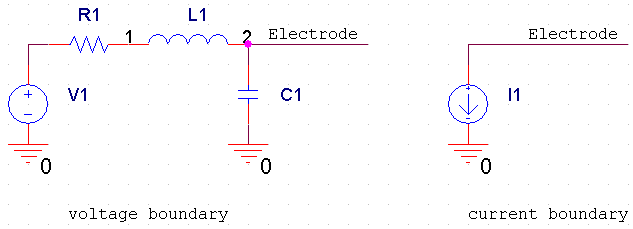
\includegraphics[scale=0.4]{electrode.png}
\caption{Voltage and current boundary.} \label{Electrode}
\end{figure}


\newpage
\section{Physical Model Interface}
GSS use a dynamic mechanician to support various materials and
physical models. Each material has a dynamic load library (.so)
which contains its physical parameters. User can modify the
parameters which can be found at \$(GSS\_DIR)/src/material and
recompile it. Experts can even offer their own physical model files.

At present, GSS has a \textbf{PMIS} statement for choosing different
mobility models and impact ionization models.

\subsubsection*{Syntax}
\begin{verbatim}
        PMIS Region=<s>  Mobility=<s>  II.Model=<s>
\end{verbatim}

\small \noindent\begin{longtable}{ccccp{7cm}}
\textbf{parameter}   & \textbf{type}    & \textbf{default} & \textbf{unit} & \textbf{description} \\
Region        & string  & -         & -    & Specifies the semiconductor region which use the following physical model.\\
Mobility      & string  & Analytic  & -    & The mobility model name.\\
II.Model      & string  & Default   & -    & The impact ionization model name.\\
\end{longtable}
\normalsize

\subsubsection*{Example}
\begin{verbatim}
        PMIS Region=Si  Mobility=Philips
        PMIS Region=Si  Mobility=Lucent  II.Model=Valdinoci
\end{verbatim}

\subsubsection*{Hint}
One can set different physical models to individual region.

GSS has implemented Analytic, Philips and Lucent mobility model for
all the supported material. The Analytic and Philips mobility model
only takes parallel field effect and they can be used within all the
four solvers. The author suggest to use these models for bipolar
device simulations. The Lucent mobility model, which considers
parallel and transverse electrical field, is an accurate model for
MOS structure. But it should work with DDML1E/DDML2E solvers in
which transverse electrical field is calculated. The Lombardi and HP
(Hewlett-Packard) mobility model only validate for Silicon. These
two mobility models include parallel and transverse electrical field
corrections and can be used for MOSFET simulation. The Hypertang
mobility model only validate for GaAs. It is reported that this
model can avoid unrealistic drain current oscillation when applied
to the simulation of GaAs MESFET.

The impact ionization model is still very limited in GSS. Only
Valdinoci model for silicon is valid at present.

\newpage
\section{Solve Specification}
\subsection{Introduction}
These statements instruct GSS core to perform user specified solution(s).


\subsection{METHOD}
The \textbf{METHOD} statement sets the solver and the parameters of
the solver. At present, GSS 0.4x has basic DDM solver(DDML1E),
lattice temperature corrected DDM solver(DDML2E) and EBML3E solver which base on
energy balance model.

\subsubsection*{Syntax}
\begin{verbatim}
        METHOD Type=(DDML1E|DDMLE2|EBML3E|QDDML1E)  Scheme=Newton
               HighFieldMobility=(On|Off)   EJModel=(On|Off)
               ImpactIonization=(On|Off)    II.Type=(EdotJ|EVector|ESide|GradQf)
               BandBandTunneling=(On|Off)
               Fermi=(On|Off)
               NS=(Basic|LineSearch|TrustRegion)
               LS=(SuperLU|LU|CGS|BICG|BCGS|GMRES|TFQMR)
               Damping=(BankRose|Potential|No)
               MaxIteration=<i> relative.tol=<n>
               possion.tol=<n>  elec.continuty.tol=<n>  hole.continuty.tol=<n>
               elec.energy.tol=<n> hole.energy.tol=<n>  latt.temp.tol=<n>
               electrode.tol=<n> toler.relax=<n>
               QNFactor=<n> QPFactor=<n>
\end{verbatim}

\small \noindent\begin{longtable}{ccccp{7cm}}
\textbf{parameter}   & \textbf{type}    & \textbf{default} & \textbf{unit} & \textbf{description} \\
Type              & string  & DDML1       & -    & Specifies the solver.\\
Scheme            & string  & Newton      & -    & At present, GSS only supports Newton's full iterative scheme.\\
HighFieldMobility & bool    & On          & -    & Specifies if high field mobility should be used. GSS set this flag to OFF for equilibrium state.\\
EJModel           & bool    & Off         & -    & Specifies if EdotJ and EcrossJ should be use to calculate high field mobility.
                                                   GSS will use a simpler model when this flag is set to OFF.\\
ImpactIonization  & bool    & Off         & -    & Specifies if impact ionization should be considered.\\
II.Type           & string  & GradQf      & -    & Specifies the implement model of impact ionization. \\
BandBandTunneling & string  & Off         & -    & Specifies if band to band tunneling should be considered.\\
Fermi             & bool    & Off         & -    & Specifies if Fermi-Dirac statistics should be considered.\\
NS                & string  &LineSearch   & -    & Specifies the nonlinear solver. \\
LS                & string  &GMRES        & -    & Specifies the linear solver. \\
Damping           & string  & No          & -    & Load a Newton damping method for LineSearch or Basic Newton nonlinear solver.\\
MaxIteration      & integer & 30          & -    & The max number of iteration nonlinear solver will try. But for equilibrium state calculation, the max
                                                    allowed iteration number is 10 times more than this value.\\
relative.tol      & number  & 1e-5        & -    & When relative error of solution variable less than this value, solution is considered converged.\\
possion.tol       & number  & 1e-26       &$\rm{C\cdot {\mu m}^{-1}} $ & The absolute converged criteria for the Poisson equation.\\
elec.continuty.tol& number  & 5e-18       &$\rm{A\cdot {\mu m}^{-1}} $ & The absolute converged criteria for the electron continuity equation.\\
hole.continuty.tol& number  & 5e-18       &$\rm{A\cdot {\mu m}^{-1}} $ & The absolute converged criteria for the hole continuity equation.\\
elec.energy.tol   & number  & 1e-18       &$\rm{W\cdot {\mu m}^{-1}} $ & The absolute converged criteria for the electron energy balance equation.\\
hole.energy.tol   & number  & 1e-18       &$\rm{W\cdot {\mu m}^{-1}} $ & The absolute converged criteria for the hole energy balance equation.\\
latt.temp.tol     & number  & 1e-11       &$\rm{W\cdot {\mu m}^{-1}} $ & The absolute converged criteria for the lattice heat equation equation.\\
electrode.tol     & number  & 1e-9        &$\rm{V}$                    & The absolute converged criteria for the electrode bias equation.\\
toler.relax       & number  & 1e4         & -                          & When relative error is used as converged criteria, the equation norm should
                                                                         satisfy the absolute converged criteria with a relaxation of this value.\\
QNFactor          & number  & 1.0         & -                          & The damping quantity of electron quantum potential.\\
QPFactor          & number  & 1.0         & -                          & The damping quantity of hole quantum potential.\\
\end{longtable}
\normalsize

\subsubsection*{Example}
\begin{verbatim}
        METHOD   Type=DDML1E   Scheme=Newton  NS=LineSearch  LS=GMRES
        METHOD   Type=DDML1E   Scheme=Newton  NS=TrustRegion LS=LU
        METHOD   Type=DDML2E   Scheme=Newton  NS=Basic LS=TFGMR Damping=Potential
\end{verbatim}

\subsubsection*{Hint}
All the DDML1E/DDML2E/EBML3E/QDDML1E solvers support parallel and
transverse electrical field dependent mobility.

Lattice temperature equation is considered by DDML2E solver. The
EBML3E solver is based on advanced energy balance method. The
QDDML1E is a density-gradient solver which consists of quantum
correction to classical model.

The carrier generation by impact ionization and band band tunneling
is really difficult for calculation. However, DDML1E/DDML2E solvers
are carefully designed for impact ionization and band band tunneling
calculation, i.e. diode reverse breakdown simulation. Usually, the
temperature can't keep unchanged if carrier generation takes place.
As a result, DDML2E solver is highly recommend for these types of
situations. At present, EBML3E and QDDML1E solver don't support
impact ionization.

Fermi statistics is only supported by DDML1E and DDML2E solvers.

LineSearch and TrustRegion accelerating methods work well when
initial value a bit far from real solution, e.g. first time
computing. Basic Newton method should only be used when initial
value is near the true solution, e.g. dc sweep and transient
calculation.

Each nonlinear solver should have a inner linear solver. To choose a
suitable linear solver may help the convergence. The performance of
LineSearch and Basic Newton methods is good when Krylov subspace
linear solvers(CGS, BICG, BCGS, GMRES and TFQMR) are employed.
However, the TrustRegion method prefers LU factorization linear
solver to Krylov subspace linear solvers.

Newton Damping is a useful tool for helping convergence,
especially for the Basic Newton method.

QNFactor and QPFactor is used to enforce the convergence property of QDDML1E solver.
Since quantum solution differs much from classical solution near Si/SiO2 interface, setting
these two factors with small value i.e. 1e-4 and varying it gradually to 1.0, with each
step the solution can get convergence. At last, the value of QXFactor of 1.0
means that the quantum model is fully turned on and applied.

The parameters of \textbf{METHOD} statement will not be affected by previous \textbf{METHOD} statement.

The convergence is considered to be achieved when either the X norm
or the function residual norm falls below certain tolerance. When
every function's residual norm falls small than certain tolerance,
the absolute convergence is achieved. For X norm criteria, it should
fall below \textbf{relative.tol} and every function residual norm
should fit the relaxed (with the relaxation value of
\textbf{toler.relax)} absolute converged criteria.

\newpage
\subsection{SOLVE}
The \textbf{SOLVE} statement instructs GSS to perform a solution for one or more
specified bias points.

\subsubsection*{Syntax}
\begin{verbatim}
        SOLVE Type=EQUILIBRIUM
        SOLVE Type=STEADYSTATE
        SOLVE Type=DCSWEEP    VScan=<s>  [VScan=<s> ...]  [IVRecord=<s> ...]
              [IVFile=<s>]    VStart=<s> VStep=<s> VStop=<n>
        SOLVE Type=DCSWEEP    IScan=<s>  [IVRecord=<s> ...]
              [IVFile=<s>]    IStart=<s> IStep=<s> IStop=<n>
        SOLVE Type=TRANSIENT  ODE.Formula=(BDF1|BDF2) [IVRecord=<s> ...]
              [IVFile=<s>]    TStart=<n> TStep=<n> TStop=<n>
              AutoStep=<b>    Predict=<b>
\end{verbatim}

\small \noindent\begin{longtable}{ccccp{7cm}}
\textbf{parameter}   & \textbf{type}    & \textbf{default} & \textbf{unit} & \textbf{description} \\
Type          & string  & -  & -    & Specifies the Solve condition.\\
VScan         & string  & -  & -    & Specifies the voltage variational electrode boundary for DCSWEEP.\\
VStart        & number  & -  & $\mathrm{V}$    & The initial voltage for DC sweep.\\
VStep         & number  & -  & $\mathrm{V}$    & The voltage step size of DC sweep.\\
VStop         & number  & -  & $\mathrm{V}$    & The finish voltage for DC sweep.\\
IScan         & string  & -      & -    & Specifies the current variational electrode boundary for DCSWEEP.\\
IStart        & number  & -  & $\mathrm{mA}$    & The initial current for DC sweep.\\
IStep         & number  & -  & $\mathrm{mA}$    & The current step size of DC sweep.\\
IStop         & number  & -  & $\mathrm{mA}$    & The finish current for DC sweep.\\
IV.Record     & string  & -      & -    & Specifies which electrode's IV data should be recorded.
                                          User can define serval electrodes here. \\
IV.File       & string  & -      & -    & Specifies the file which contains the IV data.\\
ODE.Formula   & string  & BDF2   & -    & Specifies the time march scheme for solving the time-domain ordinary differential equation.\\
TStart        & number  & -  & $\mathrm{s}$    & The initial time for transient calculation.\\
TStep         & number  & -  & $\mathrm{s}$    & The time step size of transient calculation.\\
TStop         & number  & -  & $\mathrm{s}$    & The finish time for transient calculation.\\
AutoStep      & bool    & -  & True            & Use automatically time step control based on LTE.\\
Predict       & bool    & -  & True            & Predict initial value for next time step.\\
\end{longtable}
\normalsize

\subsubsection*{Example}
\begin{verbatim}
        SOLVE    Type=EQUILIBRIUM
        SOLVE    Type=DCSWEEP     VScan=Anode    IVRecord=Anode IVRecord=Cathode \
                 IVFile=ivfp.txt  VStart=0 VStep=1e-2 VStop=0.6
        SOLVE    Type=DCSWEEP     IScan=Anode    IVRecord=Anode IVRecord=Cathode \
                 IVFile=ivfp2.txt IStart=0.02 IStep=1e-2 IStop=1
        SOLVE    Type=TRANSIENT  IVRecord=Anode  IVFile=iv.txt \
                 TStart=0 TStep=1e-10  TStop=3e-8
\end{verbatim}

\subsubsection*{Hint}

For equilibrium state calculation, all the electrodes are set to
ground.

You can't do a DC sweep with current scan to GateContact and
InsulatorContact.

When STEADYSTATE or DCSWEEP solve is performed, transient 0 value of
the voltage(current) source will be used as the bias of each
electrode.

One can do voltage DCSWEEP with multi-electrode by specifying two or more VScan parameter.
The voltage will be assigned to each electrode during the simulation. This function is useful
for Double Gate MOS simulation.

The step size for DCSWEEP calculation will
automatically reduce to half size if last step diverged. Then it
will be multiplied by 1.1 on each step until it reaches original
step size.

TRANSIENT simulation now use automatically time step control based on LTE (local truncation error).

\newpage
\subsection{AC Sweep Solver}
In addition to DC steady state and transient analysis, GSS now
allows AC small-signal analysis as a post-processing step after a DC
solution.

\subsubsection*{Syntax}
\begin{verbatim}
        METHOD Type=DDML1AC   LS=(LU|CGS|BICG|BCGS|GMRES|TFQMR)
               HighFieldMobility=(On|Off)   EJModel=(On|Off)
               ImpactIonization=(On|Off)    II.Type=(EdotJ|EVector|ESide|GradQf)
               BandBandTunneling=(On|Off)
               Fermi=(On|Off)
        SOLVE  Type=ACSWEEP    ACScan=<s>  [IVRecord=<s> ...]
               [IVFile=<s>]    FStart=<s> FMultiple=<s> FStop=<n>   VAC=<n>
\end{verbatim}

\small \noindent\begin{longtable}{ccccp{7cm}}
\textbf{parameter}   & \textbf{type}    & \textbf{default} & \textbf{unit} & \textbf{description} \\
ACScan        & string  & -      & -    & Specifies the electrode for ACSWEEP.\\
FStart        & number  & 1e6   & $\mathrm{Hz}$    & The initial frequency for AC sweep.\\
FMultiple     & number  & 1.1   & -                & The multiplicative factor for incrementing frequency.\\
FStop         & number  & 1e9   & $\mathrm{Hz}$    & The finish frequency for AC sweep.\\
VAC           & number  & 0.0026  & $\mathrm{V}$  & The magnitude of the applied small-signal bias.\\
\end{longtable}
\normalsize

\subsubsection*{Hint}
This solver shared Jacobian Matrix with DDML1E solver. Which means
one should call it directly after DDML1E, keeping all the parameters
unchanged for \textbf{METHOD} statement. If a previous computed
result is imported, call DDML1E to do a steady-state calculation
again and run DDML1AC later.

The convergence may be difficult if frequency is very high, i.e.
nearly cut off frequency, because of the poor condition number of
Jacobian matrix.

\newpage
\subsection{EM FEM Solver}
GSS has a electromagnetic solver based on finite element method.
This solver calculates the distribution of electromagnetic field
radiated by monochrome (light) wave. The photon generated carrier
density in semiconductor region can be got at the same time.

\subsubsection*{Syntax}
\begin{verbatim}
        PHOTOGEN  WAVELEN=<n> INTENSITY=<n>  [ANGLE=<n>]  WTM=<n> WTE=<n>
                  [phase.diff=<n>] [quan.eff=<n>]
        METHOD    Type=EMFEM     [LS=LU]
        SOLVE
        LSOURCE   Type=UNIFORM   Tdelay=<n> Power=<n>
        LSOURCE   Type=PULSE     Tdelay=<n> Tr=<n> Tf=<n> Pw=<n> Pr=<n>
                  Powerhi=<n>    Powerlo=<n>
        LSOURCE   Type=LSHELL    DLL=<s> Func=<s>
\end{verbatim}

\textbf{Syntax for PHOTOGEN}
\small \noindent\begin{longtable}{ccccp{8cm}}
\textbf{ parameter}   & \textbf{type}         & \textbf{default} & \textbf{unit} & \textbf{description} \\
WAVELEN       & number  & 0.532 & $\mathrm{\mu m}$              & The wavelength of incident monochrome wave.\\
INTENSITY     & number  & 1.0   & $\mathrm{W \cdot cm^{-2}}$    & The power density of incident wave.\\
ANGLE         & number  & 90    & degree                        & The clockwise angle of the ray direction relative to the horizontal axis.\\
WTM           & number  & 1.0   & -                             & The percentage of intensity of TM model.\\
WTE           & number  & 0.0   & -                             & The percentage of intensity of TE model.\\
phase.diff    & number  & 0.0   & degree                        & The differentiation of phase angle between TE model and TM model.
                                                                  $\Delta \Phi=\Phi_{TM}-\Phi_{TE}$\\
quan.eff      & number  & 1.0   & -                             & The quantum efficiency (which means electron-hole pares generated by one photon)
                                                                  of photon generation.\\
\end{longtable}
\normalsize

\textbf{Syntax for LSOURCE}
\small \noindent\begin{longtable}{ccccp{8cm}}
\textbf{ parameter}   & \textbf{type}         & \textbf{default} & \textbf{unit} & \textbf{description} \\
Type   & string  & -     & -                             & The type of light source.\\
Tdelay & number  & 0.0   & $\mathrm{s}$                  & The delay time before the activation of the light source. \\
Tr     & number  & 1e-15 & $\mathrm{s}$                  & The rise time of the intensity of the pulse-type light source. \\
Tf     & number  & 1e-15 & $\mathrm{s}$                  & The fall time of the intensity of the pulse type light source. \\
Pw     & number  & 0     & $\mathrm{s}$                  & The pulse width of the intensity of the pulse type light source. \\
Pr     & number  & 0     & $\mathrm{s}$                  & The repetition period of the intensity of the pulse type light source. \\
Power  & number  & 1.0   & -                             & The multiply factor to photon generated carrier density.\\
Powerhi& number  & 1.0   & -                             & The higher multiply factor to photon generated carrier density. \\
Powerlo& number  & 0     & -                             & The lower multiply factor to photon generated carrier density. \\
DLL    & string  & -  & -                                & The name of dynamic library file.\\
Func   & string  & -  & -                                & The name of the function loaded from dynamic library file which calculates power coefficient.\\
\end{longtable}
\normalsize

\subsubsection*{Hint}
User need to build a vacuum region surrounding device and a PML
region surrounding vacuum region. These two region should have a
thickness of no less than one wave length.

The work flow of EMFEM solver shows as follows. GSS set its internal
solver to EMFEM when meets \textbf{METHOD} command with
\textbf{EMFEM} type. The actual solving action takes place when
meets the next \textbf{SOLVE} command. GSS will search the first
\textbf{PHOTOGEN} command in the input list, using the parameters in
this command during the solve procedure. This \textbf{PHOTOGEN}
command will be removed from input list after solving action. As a
result, user can set multi \textbf{PHOTOGEN} statements and repeat
\textbf{SOLVE} command for corresponding times to calculate several
beams of monochrome wave, during which the photon generated carrier
density will be added to previous result.

The iterative method such as GMRES usually leads to divergence when
solving FEM problem. LU factorization is highly recommend.

EMFEM only gets the photon generated carrier density. User should
set \textbf{one LSOURCE} to describe the time evolution of the light
source. The actual photon generated carrier density used in
semiconductor simulation is the original value multiplied with
\textbf{power} coefficient specified within \textbf{LSOURCE}.

When DDML1E or DDML2E solver is loaded for further simulation, the
photon generated carrier will be considered.

User can define their own light source by dynamic loaded library as
voltage or current source. Here is a template.
\begin{verbatim}
foo.c:
    double lsrc_power(double time) /* in the unit of s */
    {
       double power;
       /* calculate the power of light source */
       return power;
    }
\end{verbatim}


\newpage
\subsection{IV File Format}
GSS can generate IV record file for DC sweep, transient and AC sweep
calculations. Here is the file format for the three situations.

The file for DC sweep: The first line is begin with '\#', followed
by the name of each electrode. The remain part is the potential and
current for each electrode, each takes one column. The unit of
potential is volt and the unit of current is mA.

The file for transient calculation is nearly the same as the file
for DC sweep, besides that the first column is the time with the
unit of ps.

The file for AC sweep has the same head as above. The remaining part
is organized as follows: The first column is the frequency with the
unit of MHz. Then the IV properties of each electrode. Each
electrode takes six columns, the real, image and amplitude of
potential, followed by three columns for current.

Note: the electrode potential may not equal to the application
voltage if lumped elements take place.

\newpage
\section{File I/O}
\subsection{Introduction}
The \textbf{IMPORT} and \textbf{EXPORT} statements are used to read
and write solutions from a CGNS or TIF file. A model CGNS file only
contains semiconductor device structure while a core CGNS file has
previous solution data besides device structure. The TIF(Technology
Interchange Format) file is an ASCII file used by Synopsys Medici
software which equivalence to core CGNS file. We offer a small code
TIFTool which can open TIF file, view the mesh and solution data and
convert it to CGNS file.

\subsection{IMPORT and EXPORT}
\subsubsection*{Syntax}
\begin{verbatim}
        IMPORT  CoreFile=<s> | ModelFile=<s>
        EXPORT  CoreFile=<s>   [ AscFile=<s> ]  [ VTKFile=<s> ]
\end{verbatim}

\small \noindent\begin{longtable}{ccccp{7cm}}
\textbf{parameter}   & \textbf{type}    & \textbf{default} & \textbf{unit} & \textbf{description} \\
CoreFile      & string  & -  & -    & Write/read device structure and solution data to a CGNS file.\\
ModelFile     & string  & -  & -    & Read device structure from a CGNS file which probably crated by SGframework
                                      or converted from Medici TIF file by TIFTool.\\
AscFile       & string  & -  & -    & Write device structure and solution data to a TIF file.
                                      At present, we can't make our TIF file be accepted by Medici.\\
VTKFile       & string  & -  & -    & Write mesh and solution data to VTK file.\\
\end{longtable}
\normalsize

\subsubsection*{Example}
\begin{verbatim}
        EXPORT   CoreFile=init.cgns  AscFile=init.tif
        IMPORT   ModelFile=pn.cgns
        IMPORT   CoreFile=pn.cgns
\end{verbatim}

\subsubsection*{Hint}
VTK file is intended to be used for post process. User can use
Paraview\footnote{\href{http://www.paraview.org}{http://www.paraview.org}},
MayaVi or
VisIt\footnote{\href{http://www.llnl.gov/visit}{http://www.llnl.gov/visit}}
to open and view VTK file. Further more, CGNS file is also supported
by VisIt.


\newpage
\section{Post Process}
\subsection{Plot}
The \textbf{PLOT} statement initializes the graphical display device for two and three dimensional
plots of device characteristics(3D) and device meshes(2D).

\subsubsection*{Syntax}
\begin{verbatim}
     PlotMesh  [TIFF.Out=<s>]
     Plot  Variable=Mesh [PS.Out=<s>] [TIFF.Out=<s>]
           [Resolution=(RES.Low|RES.Middle|RES.High)]
     Plot  Variable=(Na|Nd|ElecDensity|HoleDensity|Potential|EFieldX|EFieldy|Temperature)
           [ Measure=(Linear|SignedLog) ]
           [ PS.Out=<s> ] [ TIFF.Out=<s> ] [ Resolution=(RES.Low|RES.Middle|RES.High) ]
           [ AzAngle=<n> ] [ ElAngle=<n> ] [ Style=(Scale|Color|GrayLevel) ]
\end{verbatim}

\small
\noindent\begin{longtable}{ccccp{7cm}}
\textbf{parameter}   & \textbf{type}    & \textbf{default} & \textbf{unit} & \textbf{description} \\
Variable      & string  & -  & -             & This parameter specifies plot context.\\
PS.OUT        & string  & -  & -             & Specifies the postscript file name. The plot window will be saved to it.\\
TIFF.OUT      & string  & -  & -             & Specifies the TIFF file name. The plot window will be saved to it.
                                               Only available for X11 system. \\
Resolution    & string  & RES.Middle  & -    & The resolution of plot window.\\
Measure       & string  & Linear &           & Specifies the data axis to be linear or logarithmic.  \\
AzAngle       & number  & 240 & $\mathrm{degree}$  & The initial azimuthal rotation angle, 0$\leq$\textbf{AzAngle}<360. \\
ElAngle       & number  & 60  & $\mathrm{degree}$  & The initial elevation rotation angle. 0$\leq$\textbf{ElAngle}<70.\\
Style         & string  & Color   & -              & The plot style. \\
\end{longtable}
\normalsize

\subsubsection*{Example}
\begin{verbatim}
        PLOT  Variable=Mesh PS.OUT=mesh.ps
        PLOT  Variable=Nd Resolution=RES.High AzAngle=240  ElAngle=40  Style=Scale
        PLOT  Variable=Potential  Resolution=RES.Middle TIFF.out=potential.tiff\
              AzAngle=240  ElAngle=40  Style=Color
\end{verbatim}

\subsubsection*{Hint}
\textbf{PlotMesh} is an interactive GUI for mesh display only exist for X11 system.

The \textbf{PLOT} command can be used on both X11 and Win32 systems.
The 3D plot can be rotated by mouse and terminated by ESC key press.
If PS.OUT or TIFF.OUT argument is specified, the latest window image will be saved.


\newpage
\subsection{Probe}
The \textbf{PROBE} statement is used to extract field data along a
user defined segment. The segment can be a boundary or a segment
pre-defined in the region. For the in-region segment, GSS will set
it as Neumann boundary with no heat flux which takes not effect to
simulation result.

\subsubsection*{Syntax}
\begin{verbatim}
     Probe  Variable=(Na|Nd|ElecDensity|HoleDensity|Potential|EFieldX|EFieldy|Temperature)
            Region=<s> Segment=<s> ProbeFile=<s> Append=<b>
\end{verbatim}

\small \noindent\begin{longtable}{ccccp{9cm}}
\textbf{parameter}   & \textbf{type}    & \textbf{default} & \textbf{unit} & \textbf{description} \\
Variable      & string  & -  & -             & This parameter specifies probe context.\\
Region        & string  & -  & -             & Specifies the region name which the segment belongs to.\\
Segment       & string  & -  & -             & Specifies the segment name for probing the data.\\
ProbeFile     & string  & -  & -             & The file name for recording the data.\\
Append        & bool    &OFF & -             & Specifies the data should be appended to the file.  \\
\end{longtable}
\normalsize

\subsubsection*{Example}
\begin{verbatim}
    PROBE  Variable=Nd         Region=Si Segment=PB1 ProbeFile=Nd.txt Append=Off
    PROBE  Variable=Potential  Region=Si Segment=PB2 ProbeFile=P.txt  Append=On
\end{verbatim}

\subsubsection*{Hint}
Each \textbf{PROBE} statement records one variable for the whole segment to a user-specified file.
GSS pushes \textbf{PROBE} statement as the sequence of input text into a stack until a
\textbf{SOLVE} statement is met. These \textbf{PROBE} statements record the data during solve process.
After that, GSS will clear the stack. In short, \textbf{PROBE} only operates for next \textbf{SOLVE} process.

The file format for probe is show as follows:
\begin{verbatim}
    #region_name segment_name
    #node_num  X   Y
    #  0       x0  y0
    #  1       x1  y1
    #  ..............
    #SOLVE_TYPE  variable_name
    [V/I/Time]       v0     v1     v2 ...
    .....................................
\end{verbatim}
The head of file is the segment information, including region name,
segment name, total node number and the location of each node. The
last line of head shows the solve type and variable name. The solve
type can be "EQUILIBRIUM", "STEADYSTATE", "DCSWEEP\_VSCAN",
"DCSWEEP\_ISCAN" and "TRANSIENT". For the last three types, GSS will
record V/I/Time in the first column, respectively. The variable
value for all the nodes are listed in the same line.

%\begin{figure}[ht]
%\centering
%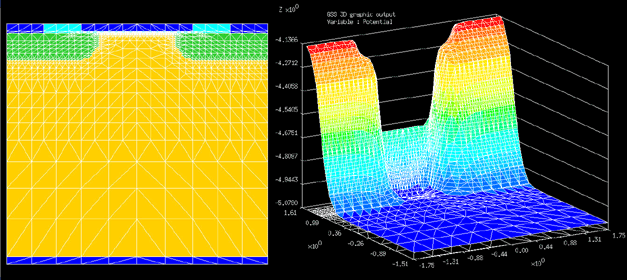
\includegraphics[scale=0.2]{plot1.png}
%\caption{2D and 3D plot.}
%\end{figure}


\newpage
\section{Convergence Problem}
The core arithmetic of GSS is solving the large scale nonlinear
equations arisen from semiconductor drift-diffusion model by
Newton's Iterative method. There are three factors which affect the
convergence of nonlinear solvers: the initial value, the Jacobian
Matrix and the inner linear solver. One must ensure that the initial
value is sufficiently near the real solution, the Jacobian Matrix is
exact or at least nearly exact and the inner linear solver can give
a suitable solution. When one of the three demands is not satisfied,
the convergence problem may raise. However, several skills can help
convergence.

If the first time running failed due to bad initial value, one can
employ a transient solver to do a time evolved solution. Set time
step to a few ps, and the solution on every step may get
convergence. After some certain steps, the initial shock is damped
and physical variables are forced to get close to real quantities.
Then the steady-state solver may work and you can get the
equilibrium solution.

Since version 0.46, GSS use automatically differentiation to
calculate Jacobian matrix. In most situations, author can guarantee
that Jacobian matrix is exact, except some rigorous situations when
round-off error is un-neglectable. However, GSS offers alternative
choice, the Matrix-Free method to set Jacobian Matrix by finite
difference approximation. This choice can be invoked with the
command line option \textit{-snes\_mf\_operator}. The Matrix-Free
method works well when impact ionization takes place, but it runs
much slower than original method.

Sometimes the LineSearch method may failed due to bad search
direction. If one get divergence message during DC sweep and
transient simulation when using LineSearch method, one can try
TrustRegion or basic Newton method.

Newton damping is a powerful tool to help convergence. It can work
with LineSearch and Basic Newton solvers. GSS has two damping
method, BankRose and Potential. Usually, damping Potential is better
than BankRose.

The most difficult problem is the failure of inner linear solver.
When the Jacobian Matrix is singular, problems may happen.
Especially one sets electrodes with lumped resistor or current
sources. If one get a convergence failed message for these
situations, please check the problem by adding command line option
\textit{-ksp\_monitor} to exam the convergence history. For more
information, one can use \textit{-ksp\_singmonitor} to get the
condition number of matrix (this works only with GMRES method).

The author suggests some method to overcome the problem. First, one
may improve the condition number by enlarging the DopingScale, but
this will increase numerical error. Second, one should carefully
choose the linear solver.

Here is the introduction of the main linear solvers GSS can use.
GMRES is a robust method for non-symmetric matrices. It must retain
all the previous vectors during iterative. The implemented code
often uses a "restart" method to avoid large memory requirement.
Sometimes the solution breaks when restart too often. One can
increase this restart steps by \textit{-ksp\_gmres\_restart <n>} (n
is the restart steps, default 150) BiCG and CGS often have irregular
convergence behavior. The irregular result may get things worse.
Bi-CGSTAB is the improved method to BiCG and CGS, which avoids the
irregular convergence patterns of BiCG/CGS while maintaining about
the same speed of convergence. TFQMR avoids the irregular
convergence behavior of BiCG. Also it avoids some breakdown
situations of BiCG. When BiCG temporarily stagnates or diverges,
TFQMR may still works. At last, LU factorization is the basic method
for solving linear systems. Besides build-in LU solver, PETSC can be
compiled with external LU factorization package such as SuperLU and
UMFPACK. This method works slow but usually more stable than
iteration solver.

In conclusion, LU factorization is recommend for conquering the
singular problem. But user can try GMRES with large restart steps,
Bi-CGSTAB and TFQMR methods for better efficiency.


\section{Memory and CPU requirement}
Thanks to C++'s dynamic memory manege system, GSS can solve problems
with any scale (at least, theoretically). The memory requirement is
not a serious bottleneck. A very large problem which contains 100K
nodes only requires about 300MB memory. This requirement is easy to
be satisfied with modern computers.

Because the core arithmetic of GSS is solving nonlinear equations,
which involves lots of solutions of linear system, the CPU time is
related with linear solvers, which is $O(n^3)$ with LU solver and
$O(n^2)$ with krylov iterative solver, in which $n$ is the problem
scale.

Fig\ref{CPUTime1} shows the CPU time vs node number with a PN diode
simulation by BCGS method on a Xeon 3.6GHz workstation. The time is
approximate the square of problem scale. It only requires serial
seconds when total node number less than 5000. But CPU time raises
to some minutes when node's number reach to 100K.

\begin{figure}[tbh]
\centering
\includegraphics[scale=0.2]{CPU.png}
\caption{CPU time vs problem scale} \label{CPUTime1}
\end{figure}

\appendix
\begingroup
  \makeatletter
  \let\chapter=\section
  % subsections goes into bookmarks but not toc
  \hypersetup{bookmarksopenlevel=1}
  \addtocontents{toc}{\protect\setcounter{tocdepth}{1}}
  % The \section command acts as \subsection.
  % Additionally the title is converted to lowercase except
  % for the first letter.
  \def\section{%
    \let\section\lc@subsection
    \lc@subsection
  }
  \def\lc@subsection{%
    \@ifstar{\def\mystar{*}\lc@sec}%
            {\let\mystar\@empty\lc@sec}%
  }
  \def\lc@sec#1{%
    \lc@@sec#1\@nil
  }
  \def\lc@@sec#1#2\@nil{%
    \begingroup
      \def\a{#1}%
      \lowercase{%
        \edef\x{\endgroup
          \noexpand\subsection\mystar{\a#2}%
        }%
      }%
    \x
  }
  % This file is a chapter.  It must be included in a larger document to work
% properly.

\chapter{GNU Free Documentation License}

Version 1.2, November 2002\\


 Copyright \copyright\ 2000,2001,2002  Free Software Foundation, Inc.\\
     59 Temple Place, Suite 330, Boston, MA  02111-1307  USA\\
 Everyone is permitted to copy and distribute verbatim copies
 of this license document, but changing it is not allowed.


\section*{PREAMBLE}

The purpose of this License is to make a manual, textbook, or other
functional and useful document ``free'' in the sense of freedom: to
assure everyone the effective freedom to copy and redistribute it,
with or without modifying it, either commercially or noncommercially.
Secondarily, this License preserves for the author and publisher a way
to get credit for their work, while not being considered responsible
for modifications made by others.

This License is a kind of ``copyleft'', which means that derivative
works of the document must themselves be free in the same sense.  It
complements the GNU General Public License, which is a copyleft
license designed for free software.

We have designed this License in order to use it for manuals for free
software, because free software needs free documentation: a free
program should come with manuals providing the same freedoms that the
software does.  But this License is not limited to software manuals;
it can be used for any textual work, regardless of subject matter or
whether it is published as a printed book.  We recommend this License
principally for works whose purpose is instruction or reference.


\section{APPLICABILITY AND DEFINITIONS}
\label{applicability}

This License applies to any manual or other work, in any medium, that
contains a notice placed by the copyright holder saying it can be
distributed under the terms of this License.  Such a notice grants a
world-wide, royalty-free license, unlimited in duration, to use that
work under the conditions stated herein.  The ``Document'', below,
refers to any such manual or work.  Any member of the public is a
licensee, and is addressed as ``you''.  You accept the license if you
copy, modify or distribute the work in a way requiring permission
under copyright law.

A ``Modified Version'' of the Document means any work containing the
Document or a portion of it, either copied verbatim, or with
modifications and/or translated into another language.

A ``Secondary Section'' is a named appendix or a front-matter section of
the Document that deals exclusively with the relationship of the
publishers or authors of the Document to the Document's overall subject
(or to related matters) and contains nothing that could fall directly
within that overall subject.  (Thus, if the Document is in part a
textbook of mathematics, a Secondary Section may not explain any
mathematics.)  The relationship could be a matter of historical
connection with the subject or with related matters, or of legal,
commercial, philosophical, ethical or political position regarding
them.

The ``Invariant Sections'' are certain Secondary Sections whose titles
are designated, as being those of Invariant Sections, in the notice
that says that the Document is released under this License.  If a
section does not fit the above definition of Secondary then it is not
allowed to be designated as Invariant.  The Document may contain zero
Invariant Sections.  If the Document does not identify any Invariant
Sections then there are none.

The ``Cover Texts'' are certain short passages of text that are listed,
as Front-Cover Texts or Back-Cover Texts, in the notice that says that
the Document is released under this License.  A Front-Cover Text may
be at most 5 words, and a Back-Cover Text may be at most 25 words.

A ``Transparent'' copy of the Document means a machine-readable copy,
represented in a format whose specification is available to the
general public, that is suitable for revising the document
straightforwardly with generic text editors or (for images composed of
pixels) generic paint programs or (for drawings) some widely available
drawing editor, and that is suitable for input to text formatters or
for automatic translation to a variety of formats suitable for input
to text formatters.  A copy made in an otherwise Transparent file
format whose markup, or absence of markup, has been arranged to thwart
or discourage subsequent modification by readers is not Transparent.
An image format is not Transparent if used for any substantial amount
of text.  A copy that is not ``Transparent'' is called ``Opaque''.

Examples of suitable formats for Transparent copies include plain
ASCII without markup, Texinfo input format, \LaTeX\ input format, SGML
or XML using a publicly available DTD, and standard-conforming simple
HTML, PostScript or PDF designed for human modification.  Examples of
transparent image formats include PNG, XCF and JPG.  Opaque formats
include proprietary formats that can be read and edited only by
proprietary word processors, SGML or XML for which the DTD and/or
processing tools are not generally available, and the
machine-generated HTML, PostScript or PDF produced by some word
processors for output purposes only.

The ``Title Page'' means, for a printed book, the title page itself,
plus such following pages as are needed to hold, legibly, the material
this License requires to appear in the title page.  For works in
formats which do not have any title page as such, ``Title Page'' means
the text near the most prominent appearance of the work's title,
preceding the beginning of the body of the text.

A section ``Entitled XYZ'' means a named subunit of the Document whose
title either is precisely XYZ or contains XYZ in parentheses following
text that translates XYZ in another language.  (Here XYZ stands for a
specific section name mentioned below, such as ``Acknowledgements'',
``Dedications'', ``Endorsements'', or ``History''.)  To ``Preserve the Title''
of such a section when you modify the Document means that it remains a
section ``Entitled XYZ'' according to this definition.

The Document may include Warranty Disclaimers next to the notice which
states that this License applies to the Document.  These Warranty
Disclaimers are considered to be included by reference in this
License, but only as regards disclaiming warranties: any other
implication that these Warranty Disclaimers may have is void and has
no effect on the meaning of this License.


\section{VERBATIM COPYING}
\label{verbatim}

You may copy and distribute the Document in any medium, either
commercially or noncommercially, provided that this License, the
copyright notices, and the license notice saying this License applies
to the Document are reproduced in all copies, and that you add no other
conditions whatsoever to those of this License.  You may not use
technical measures to obstruct or control the reading or further
copying of the copies you make or distribute.  However, you may accept
compensation in exchange for copies.  If you distribute a large enough
number of copies you must also follow the conditions in
section~\ref{copying}.

You may also lend copies, under the same conditions stated above, and
you may publicly display copies.


\section{COPYING IN QUANTITY}
\label{copying}

If you publish printed copies (or copies in media that commonly have
printed covers) of the Document, numbering more than 100, and the
Document's license notice requires Cover Texts, you must enclose the
copies in covers that carry, clearly and legibly, all these Cover
Texts: Front-Cover Texts on the front cover, and Back-Cover Texts on
the back cover.  Both covers must also clearly and legibly identify
you as the publisher of these copies.  The front cover must present
the full title with all words of the title equally prominent and
visible.  You may add other material on the covers in addition.
Copying with changes limited to the covers, as long as they preserve
the title of the Document and satisfy these conditions, can be treated
as verbatim copying in other respects.

If the required texts for either cover are too voluminous to fit
legibly, you should put the first ones listed (as many as fit
reasonably) on the actual cover, and continue the rest onto adjacent
pages.

If you publish or distribute Opaque copies of the Document numbering
more than 100, you must either include a machine-readable Transparent
copy along with each Opaque copy, or state in or with each Opaque copy
a computer-network location from which the general network-using
public has access to download using public-standard network protocols
a complete Transparent copy of the Document, free of added material.
If you use the latter option, you must take reasonably prudent steps,
when you begin distribution of Opaque copies in quantity, to ensure
that this Transparent copy will remain thus accessible at the stated
location until at least one year after the last time you distribute an
Opaque copy (directly or through your agents or retailers) of that
edition to the public.

It is requested, but not required, that you contact the authors of the
Document well before redistributing any large number of copies, to give
them a chance to provide you with an updated version of the Document.


\section{MODIFICATIONS}
\label{modifications}

You may copy and distribute a Modified Version of the Document under
the conditions of sections~\ref{verbatim} and \ref{copying} above,
provided that you release
the Modified Version under precisely this License, with the Modified
Version filling the role of the Document, thus licensing distribution
and modification of the Modified Version to whoever possesses a copy
of it.  In addition, you must do these things in the Modified Version:

\renewcommand{\labelenumi}{\Alph{enumi}.}
\begin{enumerate}
\item Use in the Title Page (and on the covers, if any) a title distinct
   from that of the Document, and from those of previous versions
   (which should, if there were any, be listed in the History section
   of the Document).  You may use the same title as a previous version
   if the original publisher of that version gives permission.
\item List on the Title Page, as authors, one or more persons or entities
   responsible for authorship of the modifications in the Modified
   Version, together with at least five of the principal authors of the
   Document (all of its principal authors, if it has fewer than five),
   unless they release you from this requirement.
\item State on the Title page the name of the publisher of the
   Modified Version, as the publisher.
\item Preserve all the copyright notices of the Document.
\item Add an appropriate copyright notice for your modifications
   adjacent to the other copyright notices.
\item Include, immediately after the copyright notices, a license notice
   giving the public permission to use the Modified Version under the
   terms of this License, in the form shown in the Addendum below.
\item Preserve in that license notice the full lists of Invariant Sections
   and required Cover Texts given in the Document's license notice.
\item Include an unaltered copy of this License.
\item Preserve the section Entitled ``History'', Preserve its Title, and add
   to it an item stating at least the title, year, new authors, and
   publisher of the Modified Version as given on the Title Page.  If
   there is no section Entitled ``History'' in the Document, create one
   stating the title, year, authors, and publisher of the Document as
   given on its Title Page, then add an item describing the Modified
   Version as stated in the previous sentence.
\item Preserve the network location, if any, given in the Document for
   public access to a Transparent copy of the Document, and likewise
   the network locations given in the Document for previous versions
   it was based on.  These may be placed in the ``History'' section.
   You may omit a network location for a work that was published at
   least four years before the Document itself, or if the original
   publisher of the version it refers to gives permission.
\item For any section Entitled ``Acknowledgements'' or ``Dedications'',
   Preserve the Title of the section, and preserve in the section all
   the substance and tone of each of the contributor acknowledgements
   and/or dedications given therein.
\item Preserve all the Invariant Sections of the Document,
   unaltered in their text and in their titles.  Section numbers
   or the equivalent are not considered part of the section titles.
\item Delete any section Entitled ``Endorsements''.  Such a section
   may not be included in the Modified Version.
\item Do not retitle any existing section to be Entitled ``Endorsements''
   or to conflict in title with any Invariant Section.
\item Preserve any Warranty Disclaimers.

\end{enumerate}

If the Modified Version includes new front-matter sections or
appendices that qualify as Secondary Sections and contain no material
copied from the Document, you may at your option designate some or all
of these sections as invariant.  To do this, add their titles to the
list of Invariant Sections in the Modified Version's license notice.
These titles must be distinct from any other section titles.

You may add a section Entitled ``Endorsements'', provided it contains
nothing but endorsements of your Modified Version by various
parties--for example, statements of peer review or that the text has
been approved by an organization as the authoritative definition of a
standard.

You may add a passage of up to five words as a Front-Cover Text, and a
passage of up to 25 words as a Back-Cover Text, to the end of the list
of Cover Texts in the Modified Version.  Only one passage of
Front-Cover Text and one of Back-Cover Text may be added by (or
through arrangements made by) any one entity.  If the Document already
includes a cover text for the same cover, previously added by you or
by arrangement made by the same entity you are acting on behalf of,
you may not add another; but you may replace the old one, on explicit
permission from the previous publisher that added the old one.

The author(s) and publisher(s) of the Document do not by this License
give permission to use their names for publicity for or to assert or
imply endorsement of any Modified Version.


\section{COMBINING DOCUMENTS}
\label{combining}

You may combine the Document with other documents released under this
License, under the terms defined in section~\ref{modifications}
above for modified
versions, provided that you include in the combination all of the
Invariant Sections of all of the original documents, unmodified, and
list them all as Invariant Sections of your combined work in its
license notice, and that you preserve all their Warranty Disclaimers.

The combined work need only contain one copy of this License, and
multiple identical Invariant Sections may be replaced with a single
copy.  If there are multiple Invariant Sections with the same name but
different contents, make the title of each such section unique by
adding at the end of it, in parentheses, the name of the original
author or publisher of that section if known, or else a unique number.
Make the same adjustment to the section titles in the list of
Invariant Sections in the license notice of the combined work.

In the combination, you must combine any sections Entitled ``History''
in the various original documents, forming one section Entitled
``History''; likewise combine any sections Entitled ``Acknowledgements'',
and any sections Entitled ``Dedications''.  You must delete all sections
Entitled ``Endorsements''.


\section{COLLECTIONS OF DOCUMENTS}
\label{collections}

You may make a collection consisting of the Document and other documents
released under this License, and replace the individual copies of this
License in the various documents with a single copy that is included in
the collection, provided that you follow the rules of this License for
verbatim copying of each of the documents in all other respects.

You may extract a single document from such a collection, and distribute
it individually under this License, provided you insert a copy of this
License into the extracted document, and follow this License in all
other respects regarding verbatim copying of that document.


\section{AGGREGATION WITH INDEPENDENT WORKS}
\label{aggregation}

A compilation of the Document or its derivatives with other separate
and independent documents or works, in or on a volume of a storage or
distribution medium, is called an ``aggregate'' if the copyright
resulting from the compilation is not used to limit the legal rights
of the compilation's users beyond what the individual works permit.
When the Document is included in an aggregate, this License does not
apply to the other works in the aggregate which are not themselves
derivative works of the Document.

If the Cover Text requirement of section~\ref{copying} is applicable to
these copies of the Document, then if the Document is less than one half
of the entire aggregate, the Document's Cover Texts may be placed on
covers that bracket the Document within the aggregate, or the
electronic equivalent of covers if the Document is in electronic form.
Otherwise they must appear on printed covers that bracket the whole
aggregate.


\section{TRANSLATION}
\label{translation}

Translation is considered a kind of modification, so you may
distribute translations of the Document under the terms of
section~\ref{modifications}.
Replacing Invariant Sections with translations requires special
permission from their copyright holders, but you may include
translations of some or all Invariant Sections in addition to the
original versions of these Invariant Sections.  You may include a
translation of this License, and all the license notices in the
Document, and any Warranty Disclaimers, provided that you also include
the original English version of this License and the original versions
of those notices and disclaimers.  In case of a disagreement between
the translation and the original version of this License or a notice
or disclaimer, the original version will prevail.

If a section in the Document is Entitled ``Acknowledgements'',
``Dedications'', or ``History'', the requirement
(section~\ref{modifications}) to Preserve
its Title (section~\ref{applicability}) will typically require
changing the actual title.


\section{TERMINATION}
\label{termination}

You may not copy, modify, sublicense, or distribute the Document except
as expressly provided for under this License.  Any other attempt to
copy, modify, sublicense or distribute the Document is void, and will
automatically terminate your rights under this License.  However,
parties who have received copies, or rights, from you under this
License will not have their licenses terminated so long as such
parties remain in full compliance.


\section{FUTURE REVISIONS OF THIS LICENSE}
\label{future}

The Free Software Foundation may publish new, revised versions
of the GNU Free Documentation License from time to time.  Such new
versions will be similar in spirit to the present version, but may
differ in detail to address new problems or concerns.  See
http://www.gnu.org/copyleft/.

Each version of the License is given a distinguishing version number.
If the Document specifies that a particular numbered version of this
License ``or any later version'' applies to it, you have the option of
following the terms and conditions either of that specified version or
of any later version that has been published (not as a draft) by the
Free Software Foundation.  If the Document does not specify a version
number of this License, you may choose any version ever published (not
as a draft) by the Free Software Foundation.


\section*{ADDENDUM: How to use this License for your documents}

To use this License in a document you have written, include a copy of
the License in the document and put the following copyright and
license notices just after the title page:

\begin{quote}
    Copyright \copyright\ YEAR  YOUR NAME.
    Permission is granted to copy, distribute and/or modify this document
    under the terms of the GNU Free Documentation License, Version 1.2
    or any later version published by the Free Software Foundation;
    with no Invariant Sections, no Front-Cover Texts, and no Back-Cover Texts.
    A copy of the license is included in the section entitled ``GNU
    Free Documentation License''.
\end{quote}

If you have Invariant Sections, Front-Cover Texts and Back-Cover Texts,
replace the ``with...Texts.'' line with this:

    with the Invariant Sections being LIST THEIR TITLES, with the
    Front-Cover Texts being LIST, and with the Back-Cover Texts being LIST.

If you have Invariant Sections without Cover Texts, or some other
combination of the three, merge those two alternatives to suit the
situation.

If your document contains nontrivial examples of program code, we
recommend releasing these examples in parallel under your choice of
free software license, such as the GNU General Public License,
to permit their use in free software.

\endgroup

\end{document}
